%  LaTeX support: latex@mdpi.com 
%  For support, please attach all files needed for compiling as well as the log file, and specify your operating system, LaTeX version, and LaTeX editor.

%=================================================================
\documentclass[journal,article,submit,pdftex,moreauthors]{Definitions/mdpi} 
%--------------------
% Class Options:
%--------------------
%----------
% journal
%----------
% Choose between the following MDPI journals:
% acoustics, actuators, addictions, admsci, adolescents, aerobiology, aerospace, agriculture, agriengineering, agrochemicals, agronomy, ai, air, algorithms, allergies, alloys, analytica, analytics, anatomia, animals, antibiotics, antibodies, antioxidants, applbiosci, appliedchem, appliedmath, applmech, applmicrobiol, applnano, applsci, aquacj, architecture, arm, arthropoda, arts, asc, asi, astronomy, atmosphere, atoms, audiolres, automation, axioms, bacteria, batteries, bdcc, behavsci, beverages, biochem, bioengineering, biologics, biology, biomass, biomechanics, biomed, biomedicines, biomedinformatics, biomimetics, biomolecules, biophysica, biosensors, biotech, birds, bloods, blsf, brainsci, breath, buildings, businesses, cancers, carbon, cardiogenetics, catalysts, cells, ceramics, challenges, chemengineering, chemistry, chemosensors, chemproc, children, chips, cimb, civileng, cleantechnol, climate, clinpract, clockssleep, cmd, coasts, coatings, colloids, colorants, commodities, compounds, computation, computers, condensedmatter, conservation, constrmater, cosmetics, covid, crops, cryptography, crystals, csmf, ctn, curroncol, cyber, dairy, data, ddc, dentistry, dermato, dermatopathology, designs, devices, diabetology, diagnostics, dietetics, digital, disabilities, diseases, diversity, dna, drones, dynamics, earth, ebj, ecologies, econometrics, economies, education, ejihpe, electricity, electrochem, electronicmat, electronics, encyclopedia, endocrines, energies, eng, engproc, entomology, entropy, environments, environsciproc, epidemiologia, epigenomes, est, fermentation, fibers, fintech, fire, fishes, fluids, foods, forecasting, forensicsci, forests, foundations, fractalfract, fuels, future, futureinternet, futurepharmacol, futurephys, futuretransp, galaxies, games, gases, gastroent, gastrointestdisord, gels, genealogy, genes, geographies, geohazards, geomatics, geosciences, geotechnics, geriatrics, grasses, gucdd, hazardousmatters, healthcare, hearts, hemato, hematolrep, heritage, higheredu, highthroughput, histories, horticulturae, hospitals, humanities, humans, hydrobiology, hydrogen, hydrology, hygiene, idr, ijerph, ijfs, ijgi, ijms, ijns, ijpb, ijtm, ijtpp, ime, immuno, informatics, information, infrastructures, inorganics, insects, instruments, inventions, iot, j, jal, jcdd, jcm, jcp, jcs, jcto, jdb, jeta, jfb, jfmk, jimaging, jintelligence, jlpea, jmmp, jmp, jmse, jne, jnt, jof, joitmc, jor, journalmedia, jox, jpm, jrfm, jsan, jtaer, jvd, jzbg, kidneydial, kinasesphosphatases, knowledge, land, languages, laws, life, liquids, literature, livers, logics, logistics, lubricants, lymphatics, machines, macromol, magnetism, magnetochemistry, make, marinedrugs, materials, materproc, mathematics, mca, measurements, medicina, medicines, medsci, membranes, merits, metabolites, metals, meteorology, methane, metrology, micro, microarrays, microbiolres, micromachines, microorganisms, microplastics, minerals, mining, modelling, molbank, molecules, mps, msf, mti, muscles, nanoenergyadv, nanomanufacturing,\gdef\@continuouspages{yes}} nanomaterials, ncrna, ndt, network, neuroglia, neurolint, neurosci, nitrogen, notspecified, %%nri, nursrep, nutraceuticals, nutrients, obesities, oceans, ohbm, onco, %oncopathology, optics, oral, organics, organoids, osteology, oxygen, parasites, parasitologia, particles, pathogens, pathophysiology, pediatrrep, pharmaceuticals, pharmaceutics, pharmacoepidemiology,\gdef\@ISSN{2813-0618}\gdef\@continuous pharmacy, philosophies, photochem, photonics, phycology, physchem, physics, physiologia, plants, plasma, platforms, pollutants, polymers, polysaccharides, poultry, powders, preprints, proceedings, processes, prosthesis, proteomes, psf, psych, psychiatryint, psychoactives, publications, quantumrep, quaternary, qubs, radiation, reactions, receptors, recycling, regeneration, religions, remotesensing, reports, reprodmed, resources, rheumato, risks, robotics, ruminants, safety, sci, scipharm, sclerosis, seeds, sensors, separations, sexes, signals, sinusitis, skins, smartcities, sna, societies, socsci, software, soilsystems, solar, solids, spectroscj, sports, standards, stats, std, stresses, surfaces, surgeries, suschem, sustainability, symmetry, synbio, systems, targets, taxonomy, technologies, telecom, test, textiles, thalassrep, thermo, tomography, tourismhosp, toxics, toxins, transplantology, transportation, traumacare, traumas, tropicalmed, universe, urbansci, uro, vaccines, vehicles, venereology, vetsci, vibration, virtualworlds, viruses, vision, waste, water, wem, wevj, wind, women, world, youth, zoonoticdis 
% For posting an early version of this manuscript as a preprint, you may use "preprints" as the journal. Changing "submit" to "accept" before posting will remove line numbers.

%---------
% article
%---------
% The default type of manuscript is "article", but can be replaced by: 
% abstract, addendum, article, book, bookreview, briefreport, casereport, comment, commentary, communication, conferenceproceedings, correction, conferencereport, entry, expressionofconcern, extendedabstract, datadescriptor, editorial, essay, erratum, hypothesis, interestingimage, obituary, opinion, projectreport, reply, retraction, review, perspective, protocol, shortnote, studyprotocol, systematicreview, supfile, technicalnote, viewpoint, guidelines, registeredreport, tutorial
% supfile = supplementary materials

%----------
% submit
%----------
% The class option "submit" will be changed to "accept" by the Editorial Office when the paper is accepted. This will only make changes to the frontpage (e.g., the logo of the journal will get visible), the headings, and the copyright information. Also, line numbering will be removed. Journal info and pagination for accepted papers will also be assigned by the Editorial Office.

%------------------
% moreauthors
%------------------
% If there is only one author the class option oneauthor should be used. Otherwise use the class option moreauthors.

%---------
% pdftex
%---------
% The option pdftex is for use with pdfLaTeX. Remove "pdftex" for (1) compiling with LaTeX & dvi2pdf (if eps figures are used) or for (2) compiling with XeLaTeX.

%=================================================================
% MDPI internal commands - do not modify
\firstpage{1} 
\makeatletter 
\setcounter{page}{\@firstpage} 
\makeatother
\pubvolume{1}
\issuenum{1}
\articlenumber{0}
\pubyear{2024}
\copyrightyear{2024}
%\externaleditor{Academic Editor: Firstname Lastname}
% \datereceived{ } 
% \daterevised{ } % Comment out if no revised date
% \dateaccepted{ } 
% \datepublished{ } 
%\datecorrected{} % For corrected papers: "Corrected: XXX" date in the original paper.
%\dateretracted{} % For corrected papers: "Retracted: XXX" date in the original paper.
% \hreflink{https://doi.org/} % If needed use \linebreak
%\doinum{}
%\pdfoutput=1 % Uncommented for upload to arXiv.org
%\CorrStatement{yes}  % For updates


%=================================================================
% Add packages and commands here. The following packages are loaded in our class file: fontenc, inputenc, calc, indentfirst, fancyhdr, graphicx, epstopdf, lastpage, ifthen, float, amsmath, amssymb, lineno, setspace, enumitem, mathpazo, booktabs, titlesec, etoolbox, tabto, xcolor, colortbl, soul, multirow, microtype, tikz, totcount, changepage, attrib, upgreek, array, tabularx, pbox, ragged2e, tocloft, marginnote, marginfix, enotez, amsthm, natbib, hyperref, cleveref, scrextend, url, geometry, newfloat, caption, draftwatermark, seqsplit
% cleveref: load \crefname definitions after \begin{document}
\preto{\abstractkeywords}{\nolinenumbers}

%=================================================================
% Please use the following mathematics environments: Theorem, Lemma, Corollary, Proposition, Characterization, Property, Problem, Example, ExamplesandDefinitions, Hypothesis, Remark, Definition, Notation, Assumption
%% For proofs, please use the proof environment (the amsthm package is loaded by the MDPI class).

%=================================================================
% Full title of the paper (Capitalized)
\Title{Strip It To The Bone: In-Depth Study of Facial Soft Tissue Thickness for Forensic Analysis}

%\Title{Strip It To The Bone: In-Depth Analysis of Soft Tissue Thickness for Forensic Facial Reconstruction}

% MDPI internal command: Title for citation in the left column
\TitleCitation{Strip It To The Bones: In-Depth Study of Soft Tissue Thickness for Forensic Analysis}

% Author Orchid ID: enter ID or remove command
\newcommand{\orcidauthorA}{0000-0000-0000-000X} % Add \orcidA{} behind the author's name
%\newcommand{\orcidauthorB}{0000-0000-0000-000X} % Add \orcidB{} behind the author's name

% Authors, for the paper (add full first names)
\Author{GROUP 15. Federica Amato $^{1,\dagger}$, Matteo Di Iorio $^{1,\dagger}$, Antonio Ferrigno $^{1,\dagger}$, Giulio Figliolino $^{1,\dagger}$ and Fatjona Gjikopulli $^{1,\dagger}$}

%\longauthorlist{yes}

% MDPI internal command: Authors, for metadata in PDF
\AuthorNames{Federica Amato, Matteo Di Iorio, Antonio Ferrigno, Giulio Figliolino and Fatjona Gjikopulli}

% MDPI internal command: Authors, for citation in the left column
\AuthorCitation{Amato, F.; Di Iorio, M.; Ferrigno, A.; Figliolino, G.; Gjikopulli, F.}
% If this is a Chicago style journal: Lastname, Firstname, Firstname Lastname, and Firstname Lastname.

% Affiliations / Addresses (Add [1] after \address if there is only one affiliation.)
\address{[1]
\quad Polytechnic University of Turin, Corso Duca degli Abruzzi 24, 10129 Turin, Italy; s310275@studenti.polito.it (F.A.); s316606@studenti.polito.it (M.D.I.); s316467@studenti.polito.it (A.F.); s317510@studenti.polito.it (G.F.); s317496@studenti.polito.it (F.G.)}

% Contact information of the corresponding author
% \corres{Correspondence: e-mail@e-mail.com; Tel.: (optional; include country code; if there are multiple corresponding authors, add author initials) +xx-xxxx-xxx-xxxx (F.L.)}

% Current address and/or shared authorship
% \firstnote{Current address: Affiliation.}  % Current address should not be the same as any items in the Affiliation section.
\firstnote{These authors contributed equally to this work.}
% The commands \thirdnote{} till \eighthnote{} are available for further notes

%\simplesumm{} % Simple summary

%\conference{} % An extended version of a conference paper

% Abstract (Do not insert blank lines, i.e. \\) 
\abstract{Forensic facial reconstruction is crucial for identifying human remains in a medico-legal context, but the variability in facial soft tissue thickness due to demographic factors such as age, sex, and body mass index  persists as an open problem. This study utilizes high-resolution DICOM and NRRD data to accurately measure FSTT at craniofacial landmarks, examining a sample of 57 patients (36 males, 21 females). The segmentation and mesh filtering process facilitated precise measurements. Statistical analysis using Pearson correlation coefficient and ANCOVA, along with Machine Learning models like Random Forest and Decision Trees, confirmed that BMI significantly influences FSTT. Specifically, higher BMI was found to correlate with increased FSTT, particularly in the mid-philtrum regions. Age and sex showed a lesser but still significant impact. These results confirm the importance of considering individual demographic characteristics to improve the accuracy of FFRs. This rigorous methodological approach ensures reliable and applicable results in both forensic and medical contexts, proposing a significant improvement in facial reconstruction techniques based on detailed FSTT analysis.}

% Keywords
\keyword{soft tissue thickness; DICOM data; 3D landmarks;
statistical analysis; forensic facial reconstruction; Random Forest Algorithm; ANCOVA; Linear Regression; Pearson correlation coefficient}

% The fields PACS, MSC, and JEL may be left empty or commented out if not applicable
%\PACS{J0101}
%\MSC{}
%\JEL{}

%%%%%%%%%%%%%%%%%%%%%%%%%%%%%%%%%%%%%%%%%%
% Only for the journal Diversity
%\LSID{\url{http://}}

%%%%%%%%%%%%%%%%%%%%%%%%%%%%%%%%%%%%%%%%%%
% Only for the journal Applied Sciences
%\featuredapplication{Authors are encouraged to provide a concise description of the specific application or a potential application of the work. This section is not mandatory.}
%%%%%%%%%%%%%%%%%%%%%%%%%%%%%%%%%%%%%%%%%%

%%%%%%%%%%%%%%%%%%%%%%%%%%%%%%%%%%%%%%%%%%
% Only for the journal Data
%\dataset{DOI number or link to the deposited data set if the data set is published separately. If the data set shall be published as a supplement to this paper, this field will be filled by the journal editors. In this case, please submit the data set as a supplement.}
%\datasetlicense{License under which the data set is made available (CC0, CC-BY, CC-BY-SA, CC-BY-NC, etc.)}

%%%%%%%%%%%%%%%%%%%%%%%%%%%%%%%%%%%%%%%%%%
% Only for the journal Toxins
%\keycontribution{The breakthroughs or highlights of the manuscript. Authors can write one or two sentences to describe the most important part of the paper.}

%%%%%%%%%%%%%%%%%%%%%%%%%%%%%%%%%%%%%%%%%%
% Only for the journal Encyclopedia
%\encyclopediadef{For entry manuscripts only: please provide a brief overview of the entry title instead of an abstract.}

%%%%%%%%%%%%%%%%%%%%%%%%%%%%%%%%%%%%%%%%%%
% Only for the journal Advances in Respiratory Medicine
%\addhighlights{yes}
%\renewcommand{\addhighlights}{%

%\noindent This is an obligatory section in “Advances in Respiratory Medicine”, whose goal is to increase the discoverability and readability of the article via search engines and other scholars. Highlights should not be a copy of the abstract, but a simple text allowing the reader to quickly and simplified find out what the article is about and what can be cited from it. Each of these parts should be devoted up to 2~bullet points.\vspace{3pt}\\
%\textbf{What are the main findings?}
% \begin{itemize}[labelsep=2.5mm,topsep=-3pt]
% \item First bullet.
% \item Second bullet.
% \end{itemize}\vspace{3pt}
%\textbf{What is the implication of the main finding?}
% \begin{itemize}[labelsep=2.5mm,topsep=-3pt]
% \item First bullet.
% \item Second bullet.
% \end{itemize}
%}

%%%%%%%%%%%%%%%%%%%%%%%%%%%%%%%%%%%%%%%%%%
\begin{document}

%%%%%%%%%%%%%%%%%%%%%%%%%%%%%%%%%%%%%%%%%%
\section{Introduction}
The identification of human remains has been a significant challenge for the medico-legal system. A thorough examination of recovered unidentified skeletal remains provides answers to fundamental questions regarding characteristics such as sex, age, and ethnicity, and helps to address trauma \cite{ref1}. When corpses lack distinctive features and their identities cannot be confirmed through conventional methods, such as DNA analysis, fingerprint analysis or dental records due to advanced postmortem decomposition process or insufficient information, facial reconstruction is one of the last options to recreate their antemortem appearance \citep{ref2,ref3,ref4,ref5}.
Forensic facial reconstruction (FFR) plays a crucial role in investigating victims of genocide and mass disasters, including wars, natural or intentional accidents \cite{ref4}.
The technique involves assembling an approximate soft tissue topography over the unknown skull to reconstruct its characteristics as closely as possible to the individual's appearance at the time of death \cite{ref3}. % Once the reconstruction is complete, a public campaign is launched to elicit responses about the possible identity of the remains. This is followed by a formal identification process \cite{ref3}.
% \\ Although the terms "facial reconstruction" and "facial approximation" are often used interchangeably, authors nowadays prefer "facial approximation" since it is impossible to precisely reproduce an individual's antemortem appearance.

The techniques employed to reproduce the face are method specific, which makes the overall process prone to errors. % Consequently, the practitioner can only approximate the natural appearance at best. As a result, 
Therefore FFR remains an inherently subjective and contentious process, despite incorporating complex sciences such as forensics, anthropology, osteology, and anatomy \cite{ref6}. In the 1970s, the process was manual and involved directly modelling and sculpting with clay or Plasticine on a skull model, combining soft tissue thickness with basic anatomy to reproduce faces \citep{ref7,ref8,ref9,ref10}. More recently, computerized face sculptures can be generated using specialized modelling software (digital method) \cite{ref11}.

%, with various user interfaces designed to mimic manual modelling procedures. In a 3D context, tablets and haptic devices may be used to add soft tissues to a model of the skull \cite{ref11}.
However, regardless of the method used, accurate reconstruction requires establishing parameters like facial soft tissue thickness (FSTT), which significantly impacts facial contours. % it is crucial to establish parameters and guidance such as facial soft tissue thickness (FSTT), as variations in FSTT can significantly influence the facial contours of an individual. The points used to estimate the FSTT are known as craniometric landmarks, or facial landmarks. These landmarks are key points of the face with a certain biometric and geometric significance.
FSTT measurements are based on craniometric landmarks, which are key points on the face used to estimate tissue thickness. They may be either skeletal or soft tissue-based, depending on their location: %—either on bone or directly on the skin.
 when located on bone, they are referred to as craniometric landmarks of hard tissue, while those on the skin are termed craniometric landmarks of soft tissue \citep{ref4,ref7,ref12}. % Establishing values for FSTT, as well as understanding the relationship between soft and hard tissue, can be achieved through radiological techniques such as X-ray, computed tomography (CT), nuclear magnetic resonance (NMR), and ultrasound.
 Various radiological techniques, including X-ray, computed tomography (CT), nuclear magnetic resonance (NMR) and ultrasound, are used to measure FSTT. These methods can be conducted in vivo or on cadaveric material, with the latter involving direct measurement via needle puncture \citep{ref13,ref14,ref15,ref16,ref17,ref18}.
 
Piombino et al. \cite{ref19} carried out a comprehensive analysis of FSTT, focusing on the effects of age, sex, and body mass index (BMI). Measurements were conducted on cone beam computed tomography (CBCT). % Their results revealed that BMI plays a significant role at various craniometric points, with higher BMI generally leading to increased FSTT, especially in areas like the mid-philtrum [and prosthion]. In contrast, age and sex have a more marginal yet significant/useful impact.
They found that BMI has a notable effect on FSTT, with higher BMI correlating with increased tissue thickness, particularly in the mid-philtrum. Age and sex also impact FSTT, though to a lesser extent. During the same period, the study undertaken by Park et al. \cite{ref2} involved patients with malocclusion, divided into three skeletal classes. % based on CBCT data and the ANB angle, which indicates the position of the maxilla in relation to the mandible. FSTT was compered between genders and across skeletal classes.
Key findings indicated that males generally have thicker FSTT than females across all skeletal types, aligning with previous research suggesting that testosterone promotes collagen synthesis, making men’s skin thicker.
% This aligns with previous research suggesting that men have larger bones and muscles, and testosterone promotes collagen synthesis, making men’s skin thicker.

Other studies, even older ones, focused on the same theme, yielding results that have been pivotal for subsequent research. Ellie Simpson and Maciej Henneberg \cite{ref20} investigated the relationship between facial soft tissue depths and cranial morphology in adult, white Australian cadavers. % The findings revealed significant correlations between FSTT and the size of the underlying cranial structure.
Males exhibited thicker soft tissues and larger craniometric dimensions compared to females (in accordance with the study conducted in South Korea), though there was considerable overlap of ranges. The impact of tissue embalming on FSTT was also noted, emphasizing its implications for forensic identification.

% Additionally, the study examined the impact of tissue embalming, noting significant initial increases in facial soft tissue depths due to this process. These findings hold implications for forensic identification and the estimation of facial features in extinct populations.
Another research aimed to develop a specific database for the Romanian adult population by investigating the statistical distribution and correlations of craniometric landmarks, conducted by Diac et al \cite{ref21}. % The authors categorized these landmarks by sex and weight to assist in estimating missing landmark values for unidentified bodies.
Measurements were taken on twelve landmarks from 100 cadavers. % within 24 hours of death. Results showed significant sex-related differences in one landmark and significant variations across different weight categories in seven landmarks. The study also found evidence in average FSTT compared to similar studies involving Caucasian groups from diverse geographic origins. 
Their study highlighted significant sex-related differences and variations across weight categories. The findings also contribute to a broader understanding of FSTT variations across different populations \citep{ref13,ref22,ref23,ref24,ref25}, yet consensus on this topic remains elusive.
% Indeed, in recent years, studies have shown that FSTT data can vary notably also among different population groups \citep{ref13,ref22,ref23,ref24,ref25}, yet consensus on this topic remains elusive. Thus, several countries 
%(France, Brazil, Portugal, etc.) are conducting extensive research to establish FSTT values, specific to each population \citep{ref13,ref14,ref15,ref16,ref17,ref18}.
Moritsugui et al. \cite{ref26} assessed regional differences in Brazil, finding high compatibility in FSTT averages between regions. % sought to assess the impact of regional differences within Brazil on FSTT, crucial for FFR. Researchers employed a specific CBCT protocol to standardize measurements across a sample of 101 subjects. High compatibility was observed when comparing the averages of FSTT among samples of two different geographic regions, Midwest and Southeast regions.
Regarding age groups, notable differences on the medium and inferior face were observed in females. Therefore, distinct datasets for the regions considered Brazil are unnecessary.

Despite advancements in imaging techniques and data availability, comprehensive statistical analyses on the correlation between variables such as age, sex, and BMI with FSTT, particularly using CBCT measurements, remain scarce. % there remains a scarcity of studies that have conducted comprehensive statistical analyses on the correlation between variables such as age, sex, and BMI with FSTT, particularly using CBCT measurements. Recognizing the variability in methodologies, including original measurement protocols, imaging exam sources and types, and regional chart relations, alongside the uncertain success of the FFR, poses challenges for comparing and validating results across studies. Therefore, this study advocates for further investigation into the influence of these variables on FSTT to improve the management of FFR procedures. The primary objectives include the following:
Therefore, this study advocates for further investigation into the influence of these variables on FSTT to improve the management of FFR procedures. The primary objectives are:

% This project aims to address these challenges by utilizing DICOM data to accurately measure FSTT at defined facial landmarks and perform statistical analyses to assess variations based on gender, age and BMI. The results will be benchmarked against established data to ensure reliability and validity, thereby enhancing the credibility and applicability of the findings in real-world scenarios. The primary objectives of this study include:
\begin{enumerate}
    \item Utilizing DICOM data to accurately measure FSTT at defined facial landmarks.
    
    \item Contextualizing these measurements for forensic relevance and practical use.
    
    \item Performing statistical analyses to assess FSTT variations based on gender, age, and BMI.
    
    \item Ensuring alignment of FSTT measurement accuracy with current literature for reliable comparisons and validations.
\end{enumerate}

The remaining sections of this paper are organized as follows. Section \ref{sec:matmet} elaborates on the use of high-resolution \textbf{DICOM} and \textbf{NRRD} data for accurate and reproducible measurements, detailing the statistical methods used to examine variations in FSTT. Sections \ref{sec:res} and \ref{sec:disc} present comprehensive results, discussions, and comparisons with recent studies. The final section summarizes the study's key findings, discusses its limitations, and proposes potential avenues for future research or applications.
%%%%%%%%%%%%%%%%%%%%%%%%%%%%%%%%%%%%%%%%%%
\section{Materials and Methods}
\label{sec:matmet}
The main steps that characterized the analysis will be presented, with references to the methods and strategies adopted.
\vspace{-0.35cm}
\begin{figure}[H]
\centering
\begin{minipage}{0.87\textwidth}
\centering
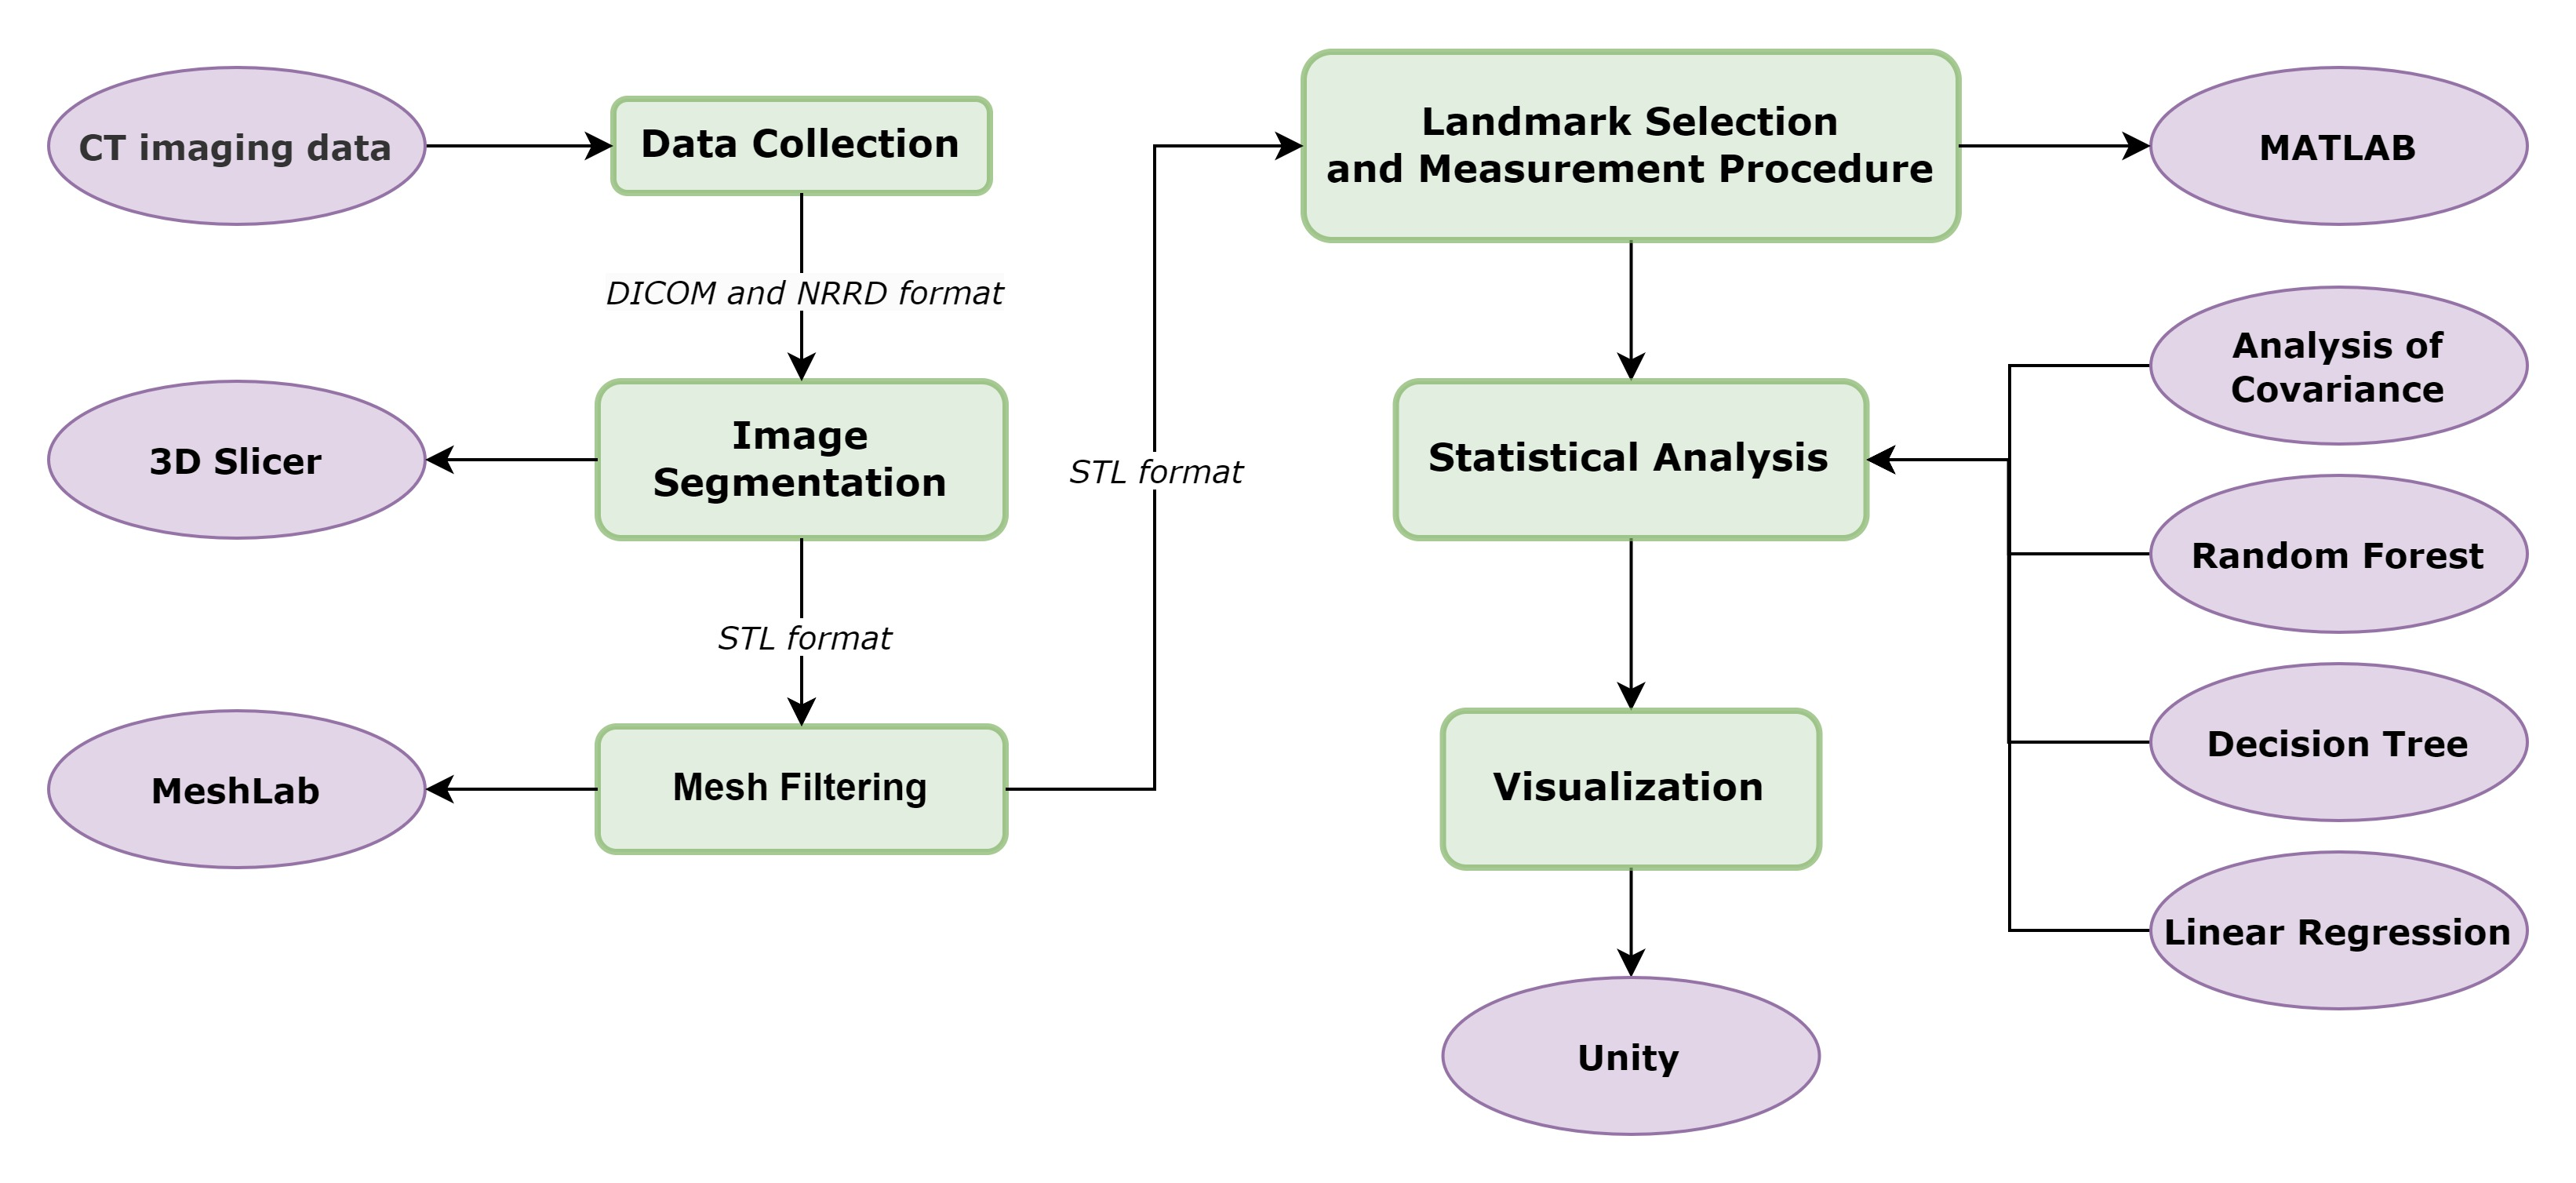
\includegraphics[width=\linewidth]{Definitions/diagramma.jpg}
\vspace{-1.1cm}
\caption{Workflow diagram.}
\label{fig1}
\end{minipage}
\end{figure}



\subsection{Data collection}

The main dataset used for this research was sourced from the publicly available collection on Academic Torrents \cite{ref27}. Specifically, this collection comprises FDG-PET/CT and radiotherapy planning CT imaging data in \textbf{DICOM} format of 298 patients from four different institutions in Québec, all with histologically proven head-and-neck cancer. All patients had pre-treatment scans between April 2006 and November 2014. Due to time constraints and the exclusion of unsuitable CT images, the analysis focused on 43 patients from the initial database, comprising 29 men and 14 women.

Furthermore, \textbf{NRRD} data from 14 patients (7 males and 7 females), provided by Professor Olivetti E.C. and Professor Marcolin F. were incorporated into the analysis. All of these patients had undergone maxillofacial surgery, and only post-operative CT scans conducted at San Giovanni Battista Hospital in Turin were considered.

\subsection{Image Segmentation and Cleaning}

The DICOM and NRRD files acquired via CBCT were 3D-modeled for the patient’s hard and soft tissues using the 3DSlicer software. To extract these tissues in 3D, the Hounsfield Unit (HU) %[value, a numerical value representing the grayscale], 
was adjusted in the Segmentation Editor section. The extracted segmentation was further refined using the \textit{Smoothing} command, which applies a Gaussian filter to smooth surfaces and reduce irregularities. Additionally, the \textit{Island} command was employed to manage and manipulate separate regions, retaining only the largest island.
% [Using “Smoothing” and “Islands” commands, the extracted segmentation was refined.
% The “Smoothing” command is used to smooth out the segmentation surfaces and reduce irregularities, which was particularly useful given the contained noise. The smoothing technique used was Gaussian, which applies a Gaussian filter to smooth the surfaces.\\
% “Islands” command is used to manage and manipulate separate regions within a segmentation. The operation used was “Keep largest island” which retains only the largest island and removes all others.]
Ultimately, the hard and soft tissue segmentations were exported in STL format for the subsequent steps.

\subsection{Mesh Filtering}

Following the import of the mesh from 3DSlicer, the model underwent a refinement process using MeshLab. Specifically, the Z-painting command was utilized to filter and select only the frontal vertices, therefore the model was exported in STL format.
%For subsequent manipulation in \textbf{Matlab}, it was not necessary to keep the entire model but only the facial shell for both tissues, so only the frontal vertices of the models were selected using the z-painting command.
% The final step in this phase was to export the  model in “.stl” format.

\subsection{Landmark Selection and Measurement Procedure}
For each patient, the further refined mesh was imported into MATLAB, and the following facial landmarks were manually identified:
\begin{itemize}
    \item Glabella
    \item Nasion
    \item Rhinion
    \item Orbitale (right and left)
    \item Orbitale superius (right and left)
    \item Zygion (right and left)
    \item Mid-philtrum (A-Point)
\end{itemize}

\begin{figure}[H]
\centering
\vspace{-0.2cm}
\begin{minipage}{0.48\textwidth}
\centering
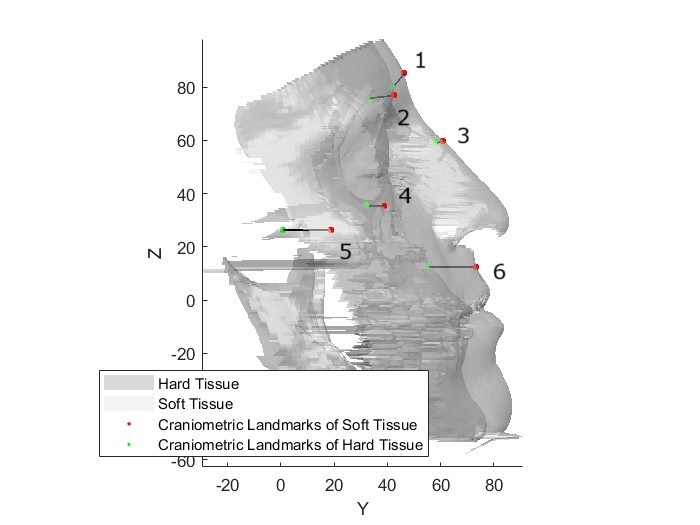
\includegraphics[width=\linewidth]{Definitions/right_num.jpg}
\caption{Right measurements: 1. Glabella, 2. Right Orbitale superius, 3. Rhinion, 4. Right Orbitale, 5. Right Zygion, 6. Mid-philtrum.}
\label{fig1}
\end{minipage}\hfill
\begin{minipage}{0.48\textwidth}
\centering
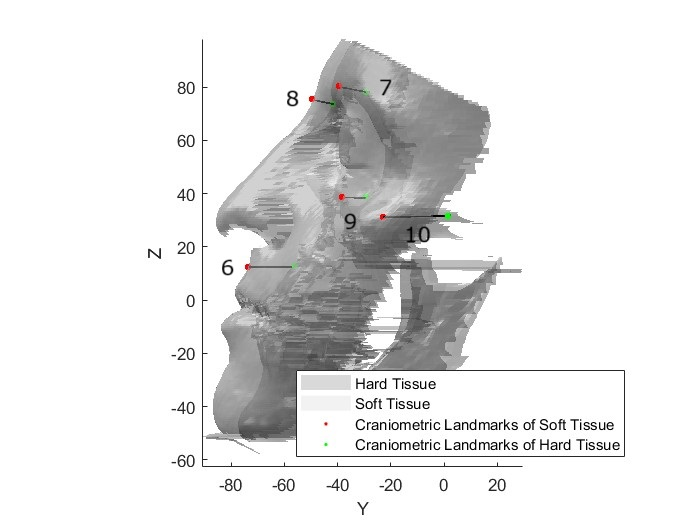
\includegraphics[width=\linewidth]{Definitions/left_num.jpg}
\caption{Left measurements: 6. Mid-philtrum, 7. Left Orbitale superius, 8. Nasion, 9. Left Orbitale, 10. Left Zygion.}
\label{fig2}
\end{minipage}
\end{figure}

\noindent These landmarks were chosen based on their relevance in craniofacial studies and their ease of identification on images. The initial goal of the analysis was to examine additional landmarks related to the lower part of the face, but due to the presence of external objects in that area, they were removed from the analysis. Each distance between corresponding landmarks on the soft tissue and hard tissue was subsequently measured and recorded for statistical analysis.

\subsection{Statistical Analysis}
\label{sec:sez2-5}

In this final part of the analysis, the main objective was to discern potential correlations between these measurements and variables such as \textbf{age} and \textbf{sex}, as well as incorporating \textbf{BMI} factors. The FSTTs from both datasets were merged for analysis, initially conducting a preliminary check for outliers and subsequently excluding them to carry out a more precise analysis. Various statistical and Machine Learning models were then employed to examine the relationship between FSTT and the aforementioned variables.

Firstly the \textbf{Pearson correlation coefficient} was used to examine the relationship between the patient age and sex with the distance of each corresponding landmark on the soft tissue and hard tissue. These insights can be valuable for identifying which landmarks are more influential in predicting demographic factors and uncovering the biological relationships underlying these variables. Moreover, they can contribute to the development of more precise predictive models.

Next, a statistical method called Analysis of Covariance (\textbf{ANCOVA}), as implemented in \cite{ref19}, was applied. To support this method, three distinct age ranges were considered:
\begin{enumerate}
    \item Under 25 ($< 25$);
    \item 25 - 60 ($\geq 25$ and $< 60$);
    \item Over 60 ($\geq 60$).
\end{enumerate}
To assess the significance of these relationships, the \textbf{p-value} was examined and used to analyze the most notable landmarks (those one with p-value $< 0.05$).

Subsequently, a \textbf{K-fold cross-validation} was conducted for both \textbf{Random Forest} (RF) and \textbf{Decision Trees} (DT) models. The analysis began by dividing the data into Training and Test Sets for each fold using a K-value of 10. Models were trained separately for predicting gender, age, and combined labels (age and gender), using \textit{RandomForestClassifier} class for RF models, and the \textit{DecisionTreeClassifier} class for DT models. Alongside accuracy computation, the importance of each predictor variable was also determined. For RF models, this was done using the \textit{features\_importances\_} parameter, while for DT models, it was done using the \textit{features\_importances\_} function.

Since the Head-Neck-CT dataset lacks BMI information, only the dataset provided by university professors was used in the subsequent statistical analysis. This approach helped evaluate relationships related to this factor and consider potential impacts on the analysis when incorporating additional information.


\newpage
\noindent In this instance, four BMI [$\frac{kg}{cm}$] ranges were taken into account: underweight ($< 18.5$), normal weight ($\geq 18.5$ and $< 24.9$), overweight ($\geq 24.9$ and $< 29.9$), obese ($\geq 29.9$), along with three age ranges:
\begin{enumerate}
    \item Under 24 ($< 24$);
    \item 24 - 29 ($\geq 24$ and $< 29$);
    \item Over 29 ($\geq 29$).
\end{enumerate}
In this scenario, the use of \textbf{Leave-One-Out} approach for RF and DF was essential since the dataset had only 14 patients. The anticipated outcomes include identifying the most significant predictor variables for each model and label type. Additionally, the analysis aims to assess the accuracy performance of each model. The specific results will be influenced by the dataset and the model configurations. For instance, 
%the number of trees in the RF models is set to 100 in this analysis, but different results could be obtained with a different number of trees. More trees lead to a more diverse set of predictions, which can result in a more stable and robust model. 
%The number is set to 100 because training a RF model involves creating multiple decision trees, each of which requires computational resources. This can be helpful to ensure that the model can be trained in a reasonable amount of time without requiring excessive computational resources.
in this analysis, RF models utilize 100 trees; however, varying this parameter could lead to different outcomes. be influenced by the dataset and the model configurations. The choice of 100 trees strikes a balance between ensuring diverse predictions and maintaining computational efficiency.

Similarly, the specific method of splitting the data into folds can also affect the results. Given the imbalanced classes in the dataset used for analysis, stratified K-fold cross-validation was the better choice.
%It works by preserving the original distribution of classes in each fold, ensuring that the proportions between classes are conserved. 
This approach ensures that each class is adequately represented across all folds, allowing for a fair and accurate evaluation of the model’s performance. This information assists in examining the correlation between FSTT and variables such as age, sex, and BMI (individually and in combination), as well as predicting the models' performance on new data.

\subsection{Visualization}

In conclusion, Unity software was utilized to visualize the obtained results.

%%%%%%%%%%%%%%%%%%%%%%%%%%%%%%%%%%%%%%%%%%
\section{Results}
\label{sec:res}


\subsection*{Mean and Standard Deviation analysis}
The estimated average FSTT and the Standard Deviation (std), categorized by subject sex, are presented in Table \ref{tab1}. Soft tissues are generally \textbf{thicker in men compared to women}, particularly at specific points such as \textbf{Orbitals} and \textbf{Zygions}.

\begin{table}[H]
\centering
\resizebox{0.525\linewidth}{!}{%
\begin{tabular}{cc|cccccc|} \cline{3-8}
 &  & \multicolumn{3}{c|}{\textbf{Men}} & \multicolumn{3}{c|}{\textbf{Women}} \\ \hline
\multicolumn{2}{|c|}{\textbf {Landmarks}} & \textit{mean} & \textit{std} & \multicolumn{1}{c|}{\textit{n}} & \textit{mean} & \textit{std} & \textit{n} \\ \hline
\multicolumn{2}{|c|}{Glabella} & 6.19 & 1.12 & \multicolumn{1}{c|} {36} & 5.95 & 1.10 & 20 \\ \hline
\multicolumn{2}{|c|}{Nasion} & 7.33 & 1.07 & \multicolumn{1}{c|}{32} & 7.15 & 1.38 & 20 \\\hline
\multicolumn{2}{|c|}{\begin{tabular}[c]{@{}c@{}}Orbitale\\ (right)\end{tabular}} & 8.52 & 2.22 & \multicolumn{1}{c|}{35} & 8.06 & 2.23 & 20 \\ \hline
\multicolumn{2}{|c|}{\begin{tabular}[c]{@{}c@{}}Orbitale \\ (left)\end{tabular}} & 8.53 & 2.31 & \multicolumn{1}{c|}{34} & 7.79 & 1.95 & 19 \\ \hline
\multicolumn{2}{|c|}{\begin{tabular}[c]{@{}c@{}}Orbitale superius\\ (right)\end{tabular}} & 8.42 & 1.61 & \multicolumn{1}{c|}{34} & 7.85 & 1.85 & 21 \\ \hline
\multicolumn{2}{|c|}{\begin{tabular}[c]{@{}c@{}}Orbitale superius\\ (left)\end{tabular}} & 8.24 & 1.82 & \multicolumn{1}{c|}{34} & 7.58 & 1.47 & 21 \\ \hline
\multicolumn{2}{|c|}{Zygion (right)} & 9.47 & 1.50 & \multicolumn{1}{c|}{32} & 9.09 & 1.14 & 20 \\ \hline
\multicolumn{2}{|c|}{Zygion (left)} & 9.78 & 1.85 & \multicolumn{1}{c|}{32} & 8.99 & 1.35 & 20 \\ \hline
\multicolumn{2}{|c|}{Rhinion} & 4.19 & 0.89 & \multicolumn{1}{c|}{30} & 3.97 & 1.09 & 18 \\ \hline
\multicolumn{2}{|c|}{\begin{tabular}[c]{@{}c@{}}Mid-philtrum/\\ A-Point\end{tabular}} & 13.99 & 2.34 & \multicolumn{1}{c|}{36} & 13.48 & 2.45 & 21 \\\hline
\end{tabular}%
}
\vspace{0.1cm}
\caption{Mean and Standard Deviation of FSTT for men and women. \label{tab1}}
\end{table}
\vspace{-0.5cm}

\noindent Figures \ref{fig4} and \ref{fig5} depict the trend of average FSTT for men and women, respectively, across three age groups (Under 25, 25-60, Over 60). It appears that the thickness of certain landmarks tends to \textbf{increase with age within both sexes}.

\begin{figure}[H]
\begin{minipage}{0.52\textwidth}
\centering
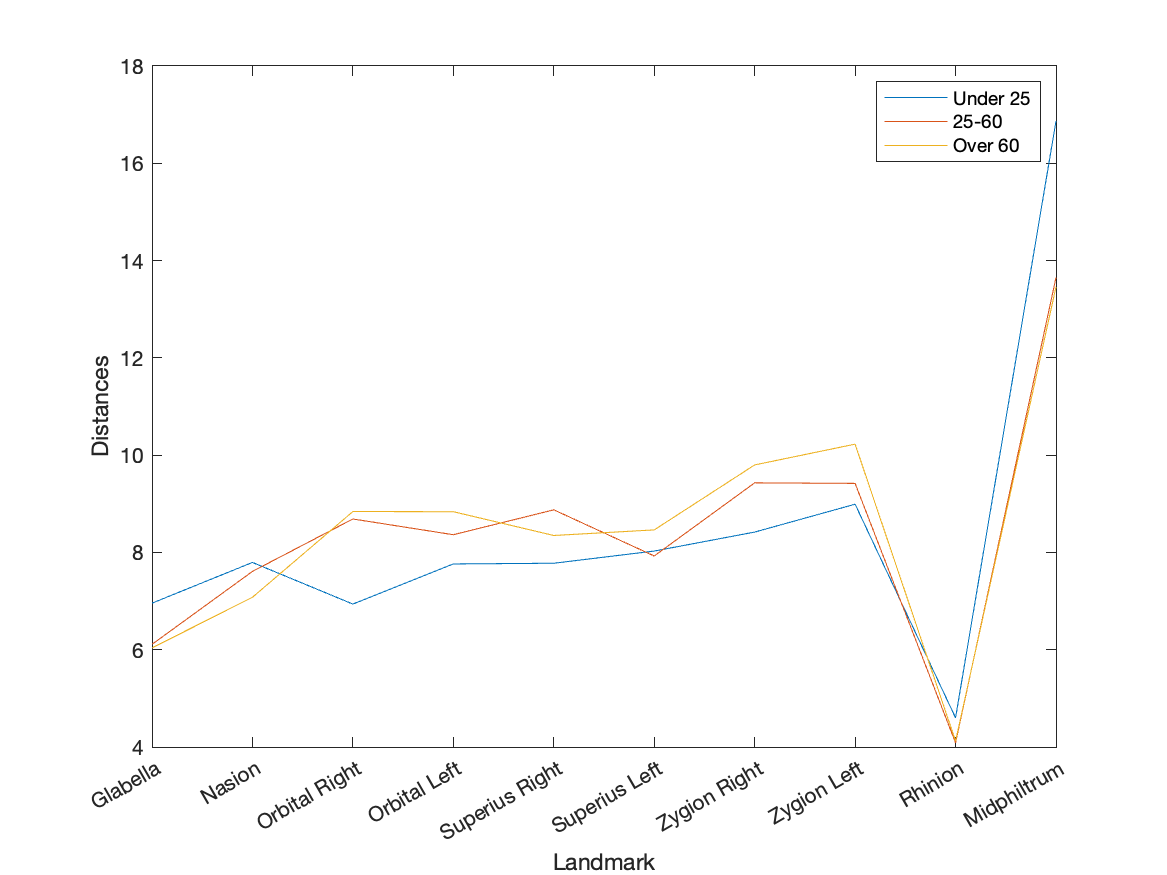
\includegraphics[width=1\linewidth]{Definitions/Men_distances_after_cleaning.png}
\caption{Mean of FSTT for men.}
\label{fig4}
\end{minipage}%
\begin{minipage}{0.52\textwidth}
\centering
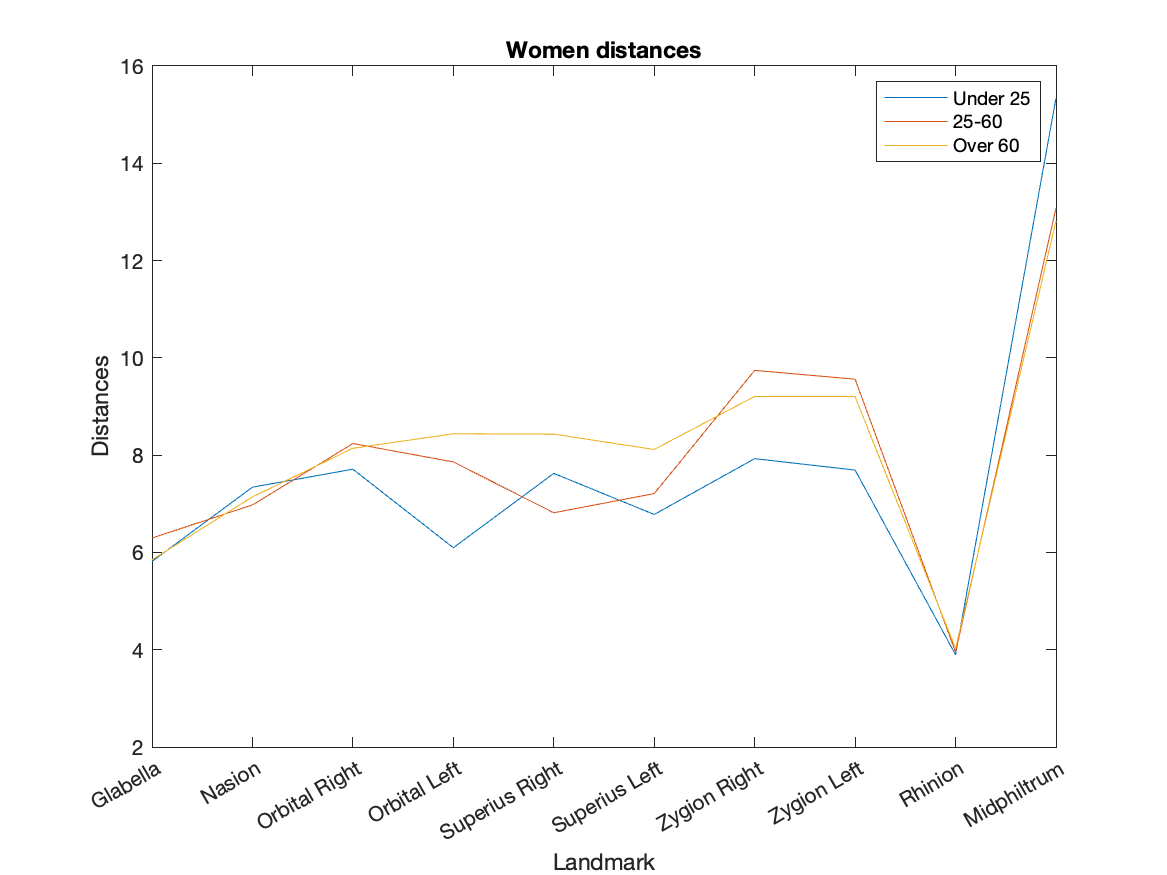
\includegraphics[width=1\linewidth]{Definitions/Women_distances_after_cleaning.png}
\caption{Mean of FSTT for women.}
\label{fig5}
\end{minipage}
\end{figure}
\noindent Considering the overall trend of FSTT for men and women, it seems that the points releated to facial medial points-specifically \textbf{Glabella}, \textbf{Rhinion} and \textbf{Mid-philtrum} are relatively thicker in men across all age groups. However, both male and female FSTT exhibit a fluctuating pattern of increase and decrease with age.

\subsection*{Linear Regression}

The linear regression models used for predicting age, sex, and age bins of individuals demonstrated varying levels of accuracy. For age prediction, the model achieved an overall accuracy of \textbf{0.96}, indicating \textbf{high precision, recall, and F1-scores} across age groups. Notably, precision, recall, and F1-scores were \textbf{perfect for the 51-60 and over 80 age groups}.

The sex prediction model attained \textbf{perfect accuracy} (\textbf{1.00}) using all landmarks but showed \textbf{decreased accuracy} (\textbf{0.75}) when considering individual patient landmarks, particularly for class female, where precision, recall, and F1-score dropped to \textbf{0.00}.

The age bin prediction model had an overall accuracy of \textbf{0.67}, performing moderately for the 61-70 age group but poorly for other age groups. These results indicate that the models are \textbf{highly effective for predicting age and sex when considering all landmarks}, but exhibit decreased performance with individual landmarks or when predicting age bins.

\subsection*{Pearson correlation coefficient}
\label{subsec:pearson-correlation}
In the analysis conducted with Pearson correlation coefficient, also considered in \cite{ref19}, each landmark has corresponding numerical values indicating its correlation with age, gender M (presumably male), and gender F (presumably female) as shown in Table \ref{tab2}. For instance, for age correlation \textbf{Glabella} and \textbf{Rhinion} seem to have the highest positive correlation, while most other landmarks have relatively low correlations.

For gender correlation, \textbf{Mid-philtrum}, \textbf{Rhinion} and \textbf{Nasion} have the highest correlation for males (and lowest correlation for females).

\vspace{-0.05cm}
\begin{table}[H]
\centering
\begin{minipage}{0.42\textwidth}
\centering
\resizebox{\linewidth}{!}{%
\begin{tabular}{clccc}
\hline
\multicolumn{2}{c}{} & \multicolumn{3}{c}{\textbf{Correlation}} \\\hline
\multicolumn{2}{c}{\textbf{Landmarks}} & \textit{age} & \textit{M} & \textit{F} \\ \hline
\multicolumn{2}{c|}{Glabella} & \textbf{0.159} & 0.186 & -0.186 \\\hline 
\multicolumn{2}{c|}{Nasion} & 0.049 & \textbf{0.224} & \textbf{-0.224} \\ \hline
\multicolumn{2}{c|}{\begin{tabular}[c]{@{}c@{}}Orbitale\\ \end{tabular}} & 0.111 & -0.199 & 0.199 \\ \hline
\multicolumn{2}{c|}{\begin{tabular}[c]{@{}c@{}}Orbitale superius\\ \end{tabular}} & 0.103 & 0.139 & -0.139 \\ \hline

\multicolumn{2}{c|}{Zygion} & 0.020 & 0.164 & -0.164 \\ \hline

\multicolumn{2}{c|}{Rhinion} & \textbf{0.170} & \textbf{0.233} & \textbf{-0.233} \\ \hline
\multicolumn{2}{c|}{\begin{tabular}[c]{@{}c@{}}Mid-philtrum/\\ A-Point\end{tabular}} & -0.028 & \textbf{0.361} & \textbf{-0.361} \\\hline
\end{tabular}%
}
\caption{Pearson correlation coefficient. \label{tab2}}
\end{minipage}\hfill
\begin{minipage}{0.42\textwidth}
\centering
\resizebox{\linewidth}{!}{%
\begin{tabular}{clccc}
\hline
\multicolumn{2}{c}{} & \multicolumn{3}{c}{\textbf{p-values}} \\ \hline
\multicolumn{2}{c|}{\textbf{Landmarks}} & \textit{gender} & \textit{age} & \textit{gender+age} \\ \hline
\multicolumn{2}{c|}{Glabella} & 0.371 & 0.510 & 0.332 \\ \hline
\multicolumn{2}{c|}{Nasion} & 0.368 & 0.683 & 0.773 \\ \hline
\multicolumn{2}{c|}{Orbitale (right)} & 0.599 & 0.323 & 0.675 \\ \hline
\multicolumn{2}{c|}{Orbitale (left)} & 0.298 & 0.165 & 0.749 \\ \hline
\multicolumn{2}{c|}{\begin{tabular}[c]{@{}c@{}}Orbitale superius\\ (right)\end{tabular}} & 0.277 & 0.619 & 0.164 \\ \hline
\multicolumn{2}{c|}{\begin{tabular}[c]{@{}c@{}}Orbitale superius\\ (left)\end{tabular}} & 0.202 & 0.281 & 0.771 \\ \hline
\multicolumn{2}{c|}{Zygion (right)} & 0.223 & {\color[HTML]{FE0000} 0.010} & 0.814 \\ \hline
\multicolumn{2}{c|}{Zygion (left)} & 0.169 & 0.132 & 0.528 \\ \hline
\multicolumn{2}{c|}{Rhinion} & 0.09 & 0.369 & 0.420 \\ \hline
\multicolumn{2}{c|}{\begin{tabular}[c]{@{}c@{}}Mid-philtrum/\\ A-Point\end{tabular}} & 0.193 & {\color[HTML]{FE0000} 0.001} & 0.839 \\ \hline
\end{tabular}%
}
\caption{p-value for ANCOVA analysis (significant p-value: $< 0.05$). \label{tab3}}
\end{minipage}
\end{table}
\vspace{-0.4cm}

\subsection*{ANCOVA and RF analysis} \label{subsec:ancova-rf-analysis}

Subsequently, ANCOVA statistical analysis was performed, with the results summerized in Table \ref{tab3}. Significant values were found only for age analysis for \textbf{right Zygion} and \textbf{Mid-philtrum} landmarks.

The final analysis, which took into account both age and sex of the patients, used two classification models: RF and DT. Only the results of the most performant model (RF) are shown in Figure {\ref{fig:fig6}}. This analysis identified which landmarks, based on their thicknesses, most influenced the classification of age, gender, and the combination of age and gender. 

From the figures, it is evident that for gender classification, the three most significant landmarks turn out to be \textbf{Nasion}, \textbf{right Orbital superius} and \textbf{right Zygion}. 
For age classification, the top three landmarks are \textbf{right Orbital}, \textbf{left Orbital} and \textbf{Mid-philtum}.
When considering the combination of gender and age, the top three landmarks turn out to be \textbf{left Orbital}, \textbf{right Zygion} and \textbf{Mid-philtrum}.

\vspace{-0.1cm}
\begin{figure}[H]
    \centering
    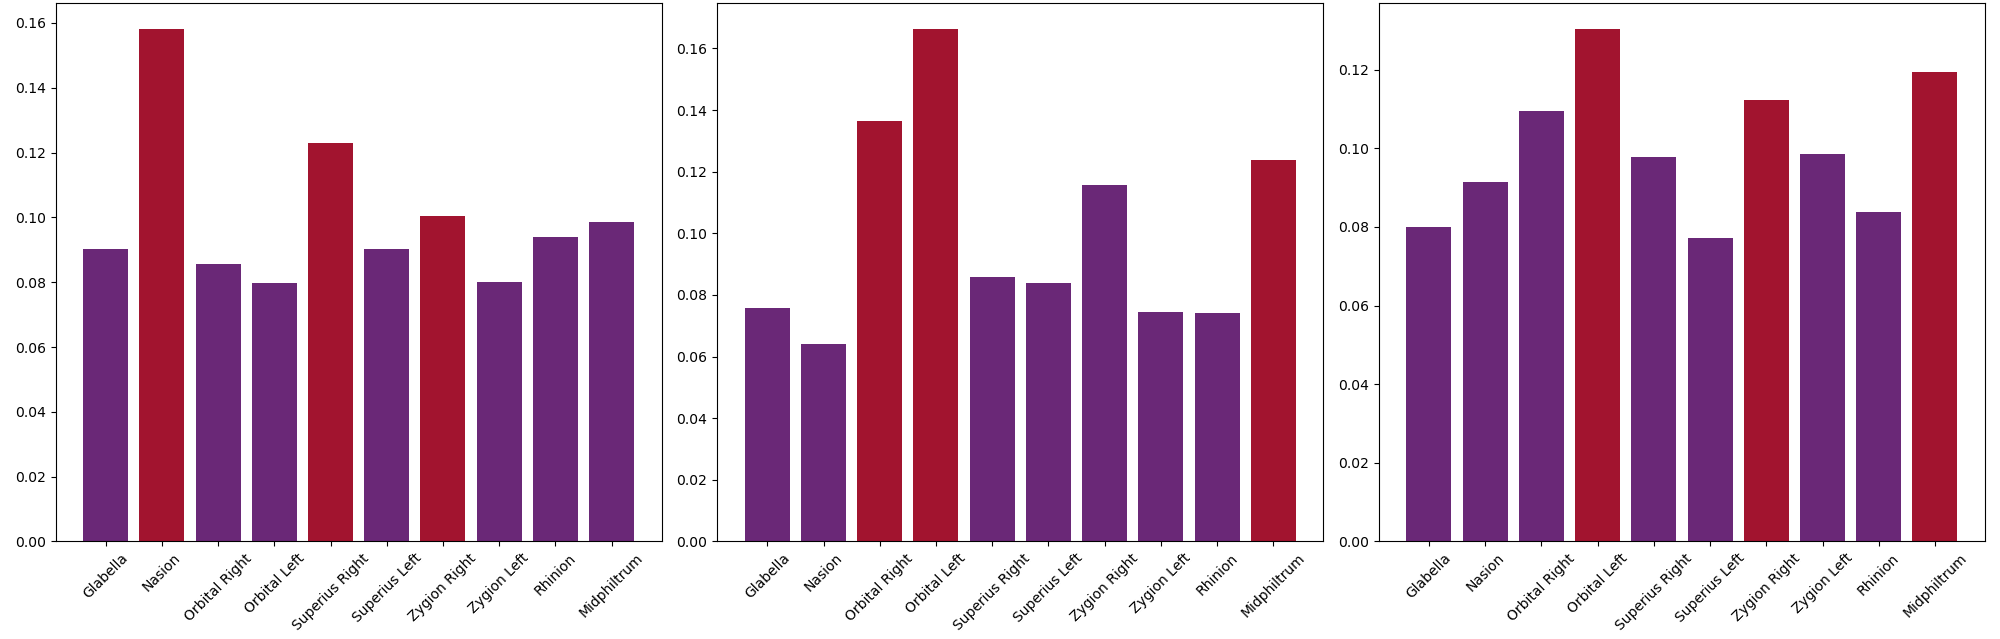
\includegraphics[width=1\linewidth]{Definitions/RF_analysis_1.png}
    \vspace{-0.5cm}
    \caption{RF analysis. From left to right: (\textbf{a}) Gender classification: accuracy of 60.00\%. (\textbf{b}) Age classification: accuracy of 60.33\%. (\textbf{c}) Combined labels classification: accuracy of 29.33\%.} 
    \label{fig:fig6}
\end{figure}

\noindent Given that the initial analysis only considered sex and age, since the Head-Neck-CT dataset does not contain information related to BMI, this final phase focused on analysing only the dataset provided by Professor Olivetti E.C. and Professor Marcolin F.. This included the BMI factor and repeated the same statistical analysis steps described previously.

It was evident that not all weight categories were covered within each age range. Consequently, the behavior of the average FSTT across different age and BMI bands was not analyzed, as the results were incomplete and thus not suitable for inclusion in the analysis.
When considering the BMI factor and distinguishing the patients by sex, the trends illustrated in Figures \ref{fig:fig7} and \ref{fig:fig8} were observed.
These figures illustrate that as weight category increases, the FSTT values tend to thicken. For example, in men, significant increases were observed at the \textbf{Zygion} and \textbf{Mid-philtrum} landmarks, while in women, the increase also encompassed the \textbf{Orbitals} and the \textbf{median points} of the face.

\vspace{-0.2cm}
\begin{figure}[H]
    \begin{minipage}{0.52\textwidth}
        \centering
        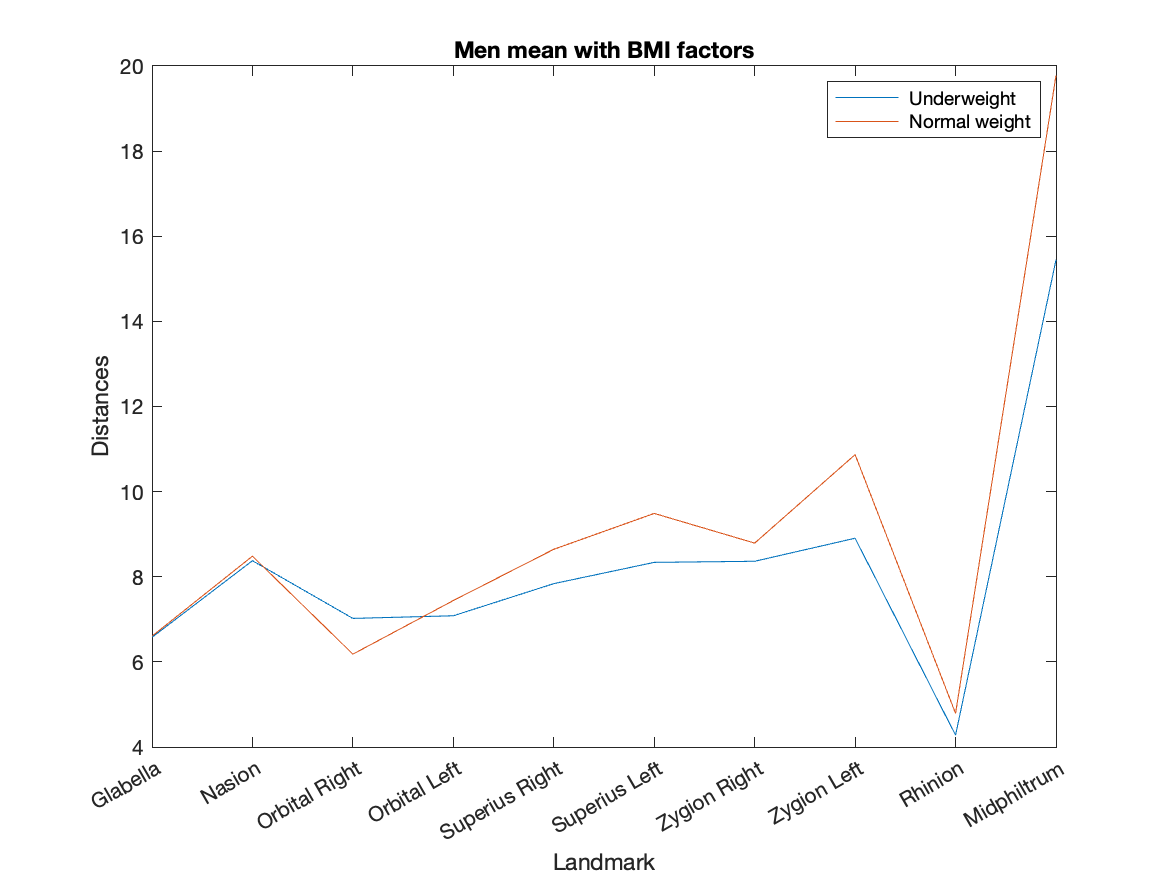
\includegraphics[width=\linewidth]{Definitions/Men_mean_BMI_withoutAge.png}
        \vspace{-0.3cm}
        \caption{Mean considering BMI ranges (men).}
        \label{fig:fig7}
    \end{minipage}
    \hfill
    \begin{minipage}{0.52\textwidth}
        \centering
        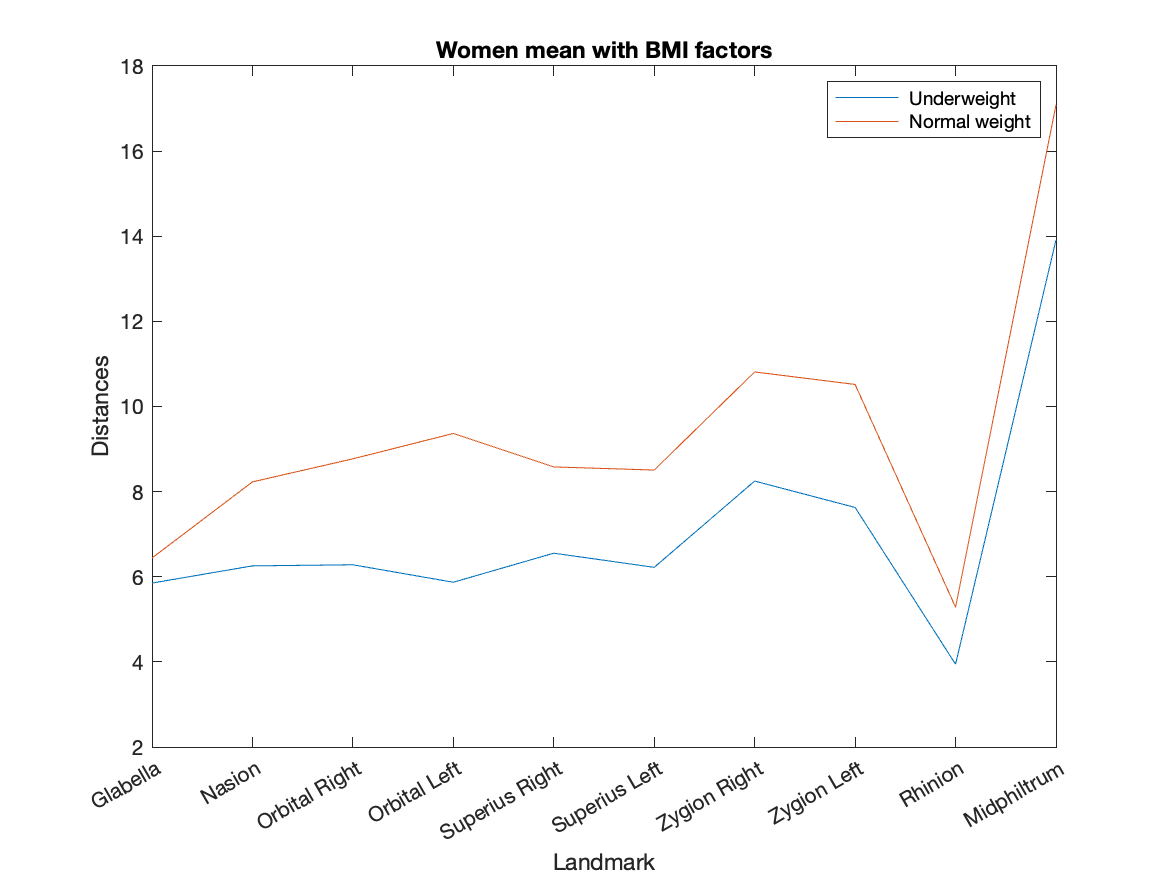
\includegraphics[width=\linewidth]{Definitions/Women_mean_BMI_withoutAge.png}
        \vspace{-0.3cm}
        \caption{Mean considering BMI ranges (women).}
        \label{fig:fig8}
    \end{minipage}
\end{figure}


Using ANCOVA analysis, the results are shown in Figure \ref{fig:fig9}. This analysis covers gender, age, BMI, the interaction between gender and BMI (\textbf{GB Interaction}), the interaction between gender and age (\textbf{GA Interaction}), the interaction between age and BMI (\textbf{AB Interaction}), and finally, the combined interaction of gender,age, and BMI combined (\textbf{GAB Interaction}). Observing this plot, it is evident that incorporating the BMI factor can enhance the analysis and yield more accurate results.

\begin{figure}[H]
    \centering
    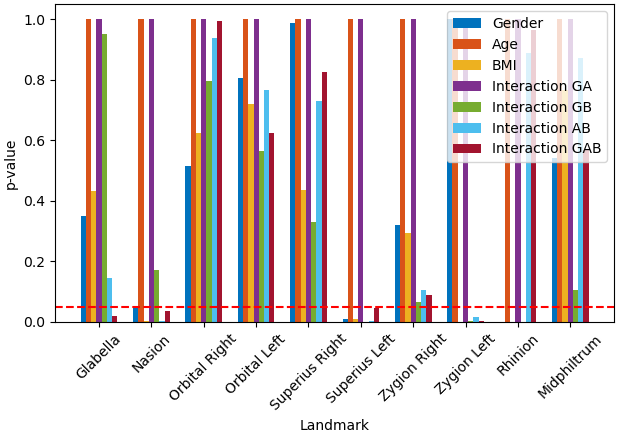
\includegraphics[width=0.6\linewidth]{Definitions/ANCOVA_BMI_after_cleaning.png}
    \vspace{-0.2cm}
    \caption{ANCOVA analysis including BMI factor.}
    \label{fig:fig9}
\end{figure}

\noindent Based on these results, it appears that the landmarks exerting the most influence are:
\begin{enumerate}
    \item \textbf{Glabella}, for GAB Interaction analysis;
    \item \textbf{Nasion}, for BMI, AB Interaction, and GAB Interaction analysis;
    \item \textbf{left Orbital Superius}, for gender, BMI, GB Interaction, AB Interaction and GAB Interaction analysis;
    \item \textbf{left Zygion}, for BMI, GB Interacion, AB Interaction and GAB Interaction analysis;
    \item \textbf{Rhinion}, for gender, BMI and GB Interaction analysis.

\end{enumerate}

Following this, the RF model was utilized, resulting in the findings depicted in Figure \ref{fig:fig10}.
As can be seen, it is evident that for BMI alone, the three most influential landmarks are \textbf{Nasion}, \textbf{right Orbiatal superius} and \textbf{left Orbital superius}. 
When considering age combined with BMI, the top three landmarks are turn out to be \textbf{Glabella}, \textbf{Nasion} and \textbf{left Orbital superius}.
In the context of gender and BMI combined, the top three landmarks are \textbf{Nasion}, \textbf{right Orbital superius} and \textbf{left Orbital superius}.
Lastly, in the interaction involving gender, age, and BMI, the three most significant landmarks turn out to be \textbf{Nasion}, \textbf{right Orbital superius} and \textbf{right Zygion}.

\begin{figure}[H]
    \centering
    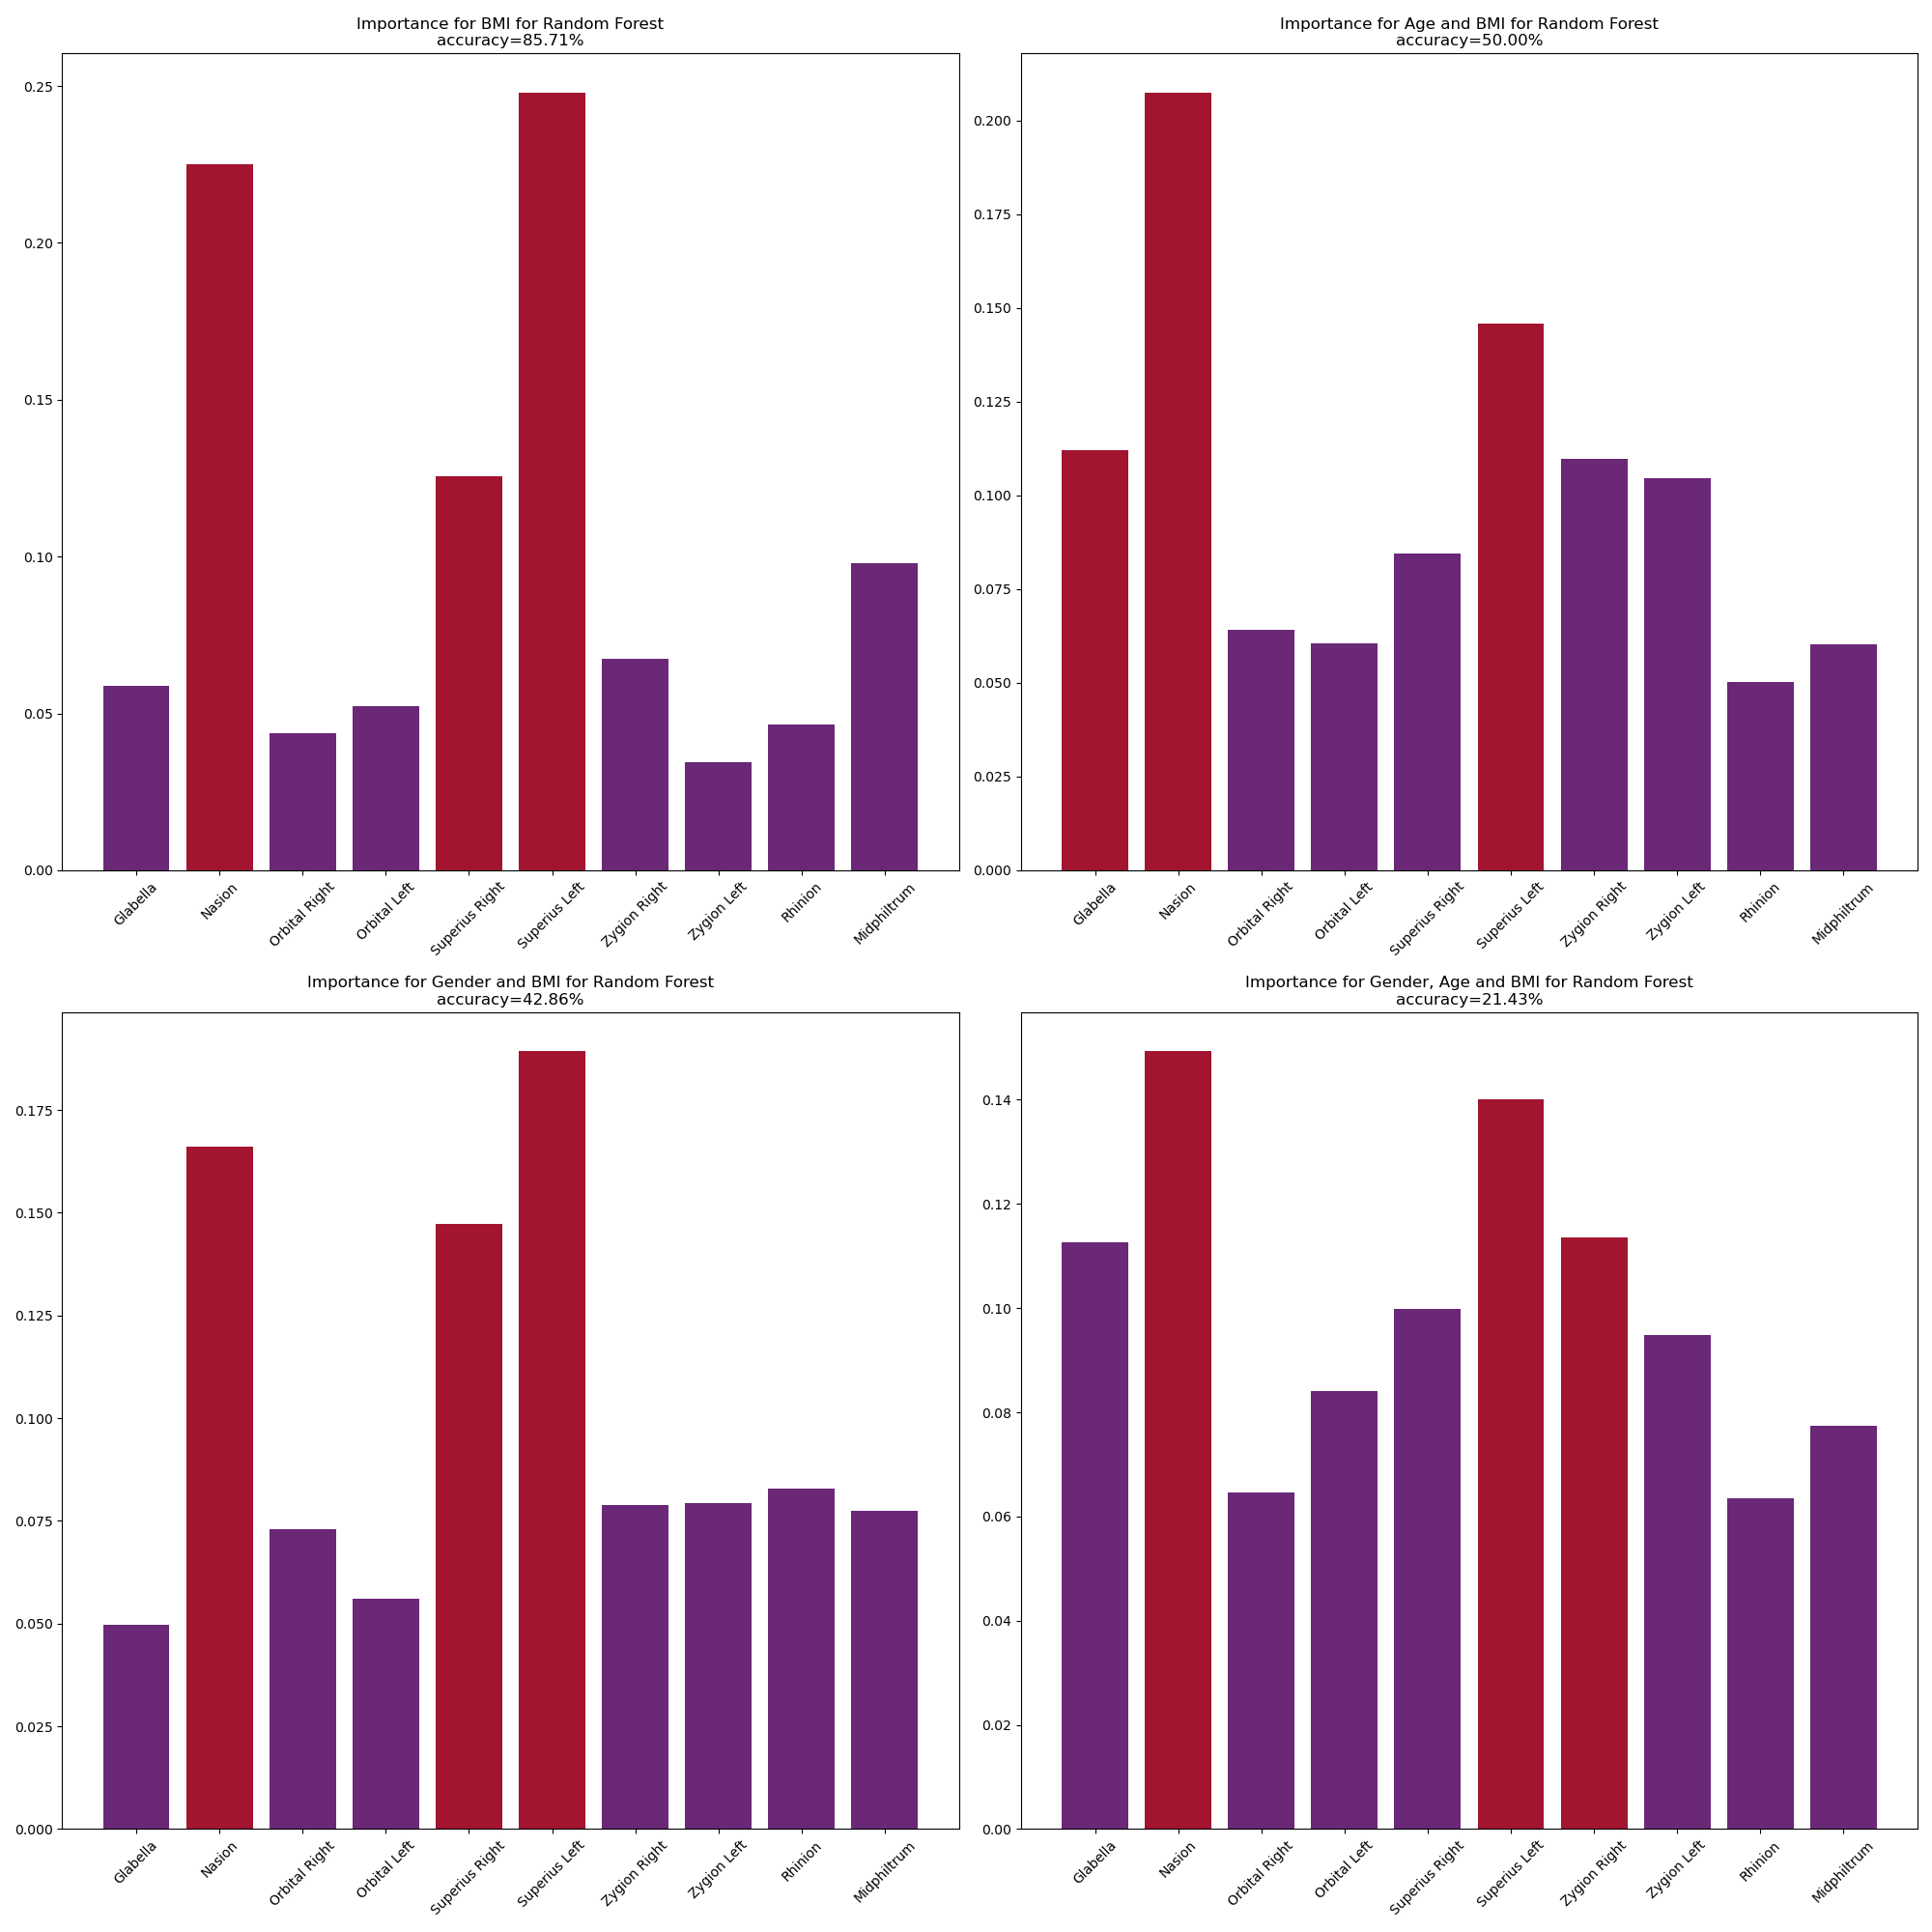
\includegraphics[width=0.9\linewidth]{Definitions/rf_bmi.png}
    \label{fig:enter-label}
\end{figure}
\begin{figure}[H]
    \centering
    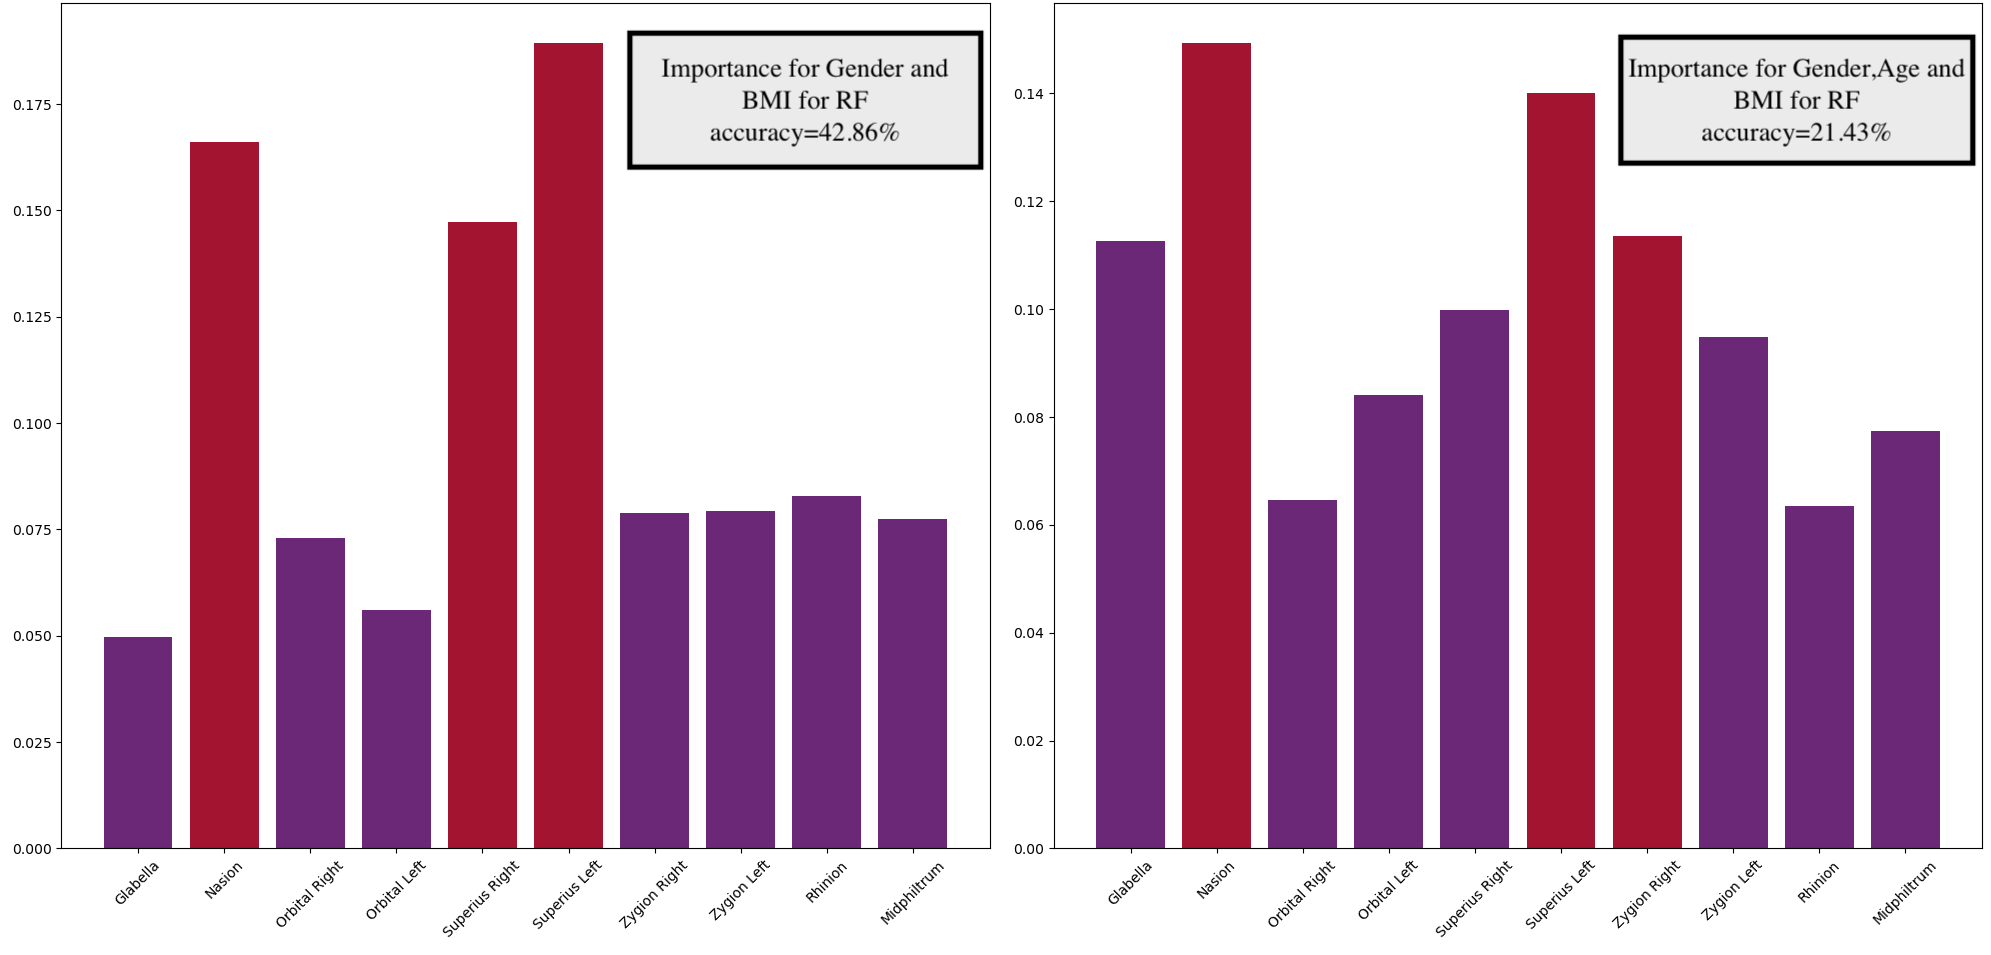
\includegraphics[width=0.9\linewidth]{{Definitions/rf_bmi copia.png}}
    \vspace{-0.2cm}
    \caption{RF analysis including BMI factor.}
    \label{fig:fig10}
\end{figure}


%%%%%%%%%%%%%%%%%%%%%%%%%%%%%%%%%%%%%%%%%%
\section{Discussion}
\label{sec:disc}
The findings of this study offer valuable insights into the impact of demographic factors on FSTT, with potential applications in FFR and related fields. Comparative analysis with previous studies reveals both similarities and differences. For instance, this study confirms the influence of age and sex on FSTT, consistent with Piombino et al. \cite{ref19}, and extends these findings through BMI analysis and other works, e.g., Codinha et al. \cite{ref1,ref13}. These correlations may depend on methodological factors such as imaging data sources and demographic diversity among study populations. Table \ref{tab4} underscores the differences in FSTT averages between genders observed in comparison with previous studies, showing thicker measurements for men at specific landmarks. Regarding age groups, there is a trend of increasing thickness with age, likely due to changes in weight distribution, though a larger sample size is needed to explore age-related variations comprehensively.

\textbf{Linear regression model} predicting age, sex, and age bins using FSTT measurements demonstrated varying levels of accuracy. The age prediction model performed exceptionally well, underscoring the potential of FSTT data for reliable age estimation. On the other hand, while the sex prediction model achieved perfect accuracy with all landmarks, it showed reduced performance with individual landmarks, emphasizing the need for comprehensive landmark analysis. The age bin prediction model exhibited limited accuracy, highlighting challenges in categorizing individuals into specific age groups based solely on FSTT measurements. These findings underscore the importance of considering multiple demographic factors and comprehensive landmark data to enhance predictive accuracy in forensic and medical applications.

\textbf{Pearson correlation coefficient} highlighted that \textbf{Glabella} and \textbf{Rhinion} landmarks as having the \textbf{highest positive correlation with age}, suggesting thicker measurements with increasing age. For gender correlation, \textbf{Mid-philtrum}, \textbf{Rhinion}, and \textbf{Nasion} landmarks showed the \textbf{strongest correlations in males} (and lowest in females), indicating gender-specific influences in these areas. Notably, \textbf{Rhinion} emerged as particularly influential for both age and gender correlations, consistent with findings by Piombino et al. \cite{ref19}.

\textbf{ANCOVA} analysis revealed that age significantly affects the thickness of the \textbf{right Zygion} and \textbf{Mid-philtrum}, suggesting these landmarks serve as indicators of age in future studies. Discrepancies from previous research may stem from the small dataset and manual landmark selection methods, affecting the precision of FSTT measurements. Incorporating BMI into the analysis highlighted \textbf{Zygion} and \textbf{Orbital superius} as notably influential in various interactions.

\textbf{RF} analysis identified distinct influential landmarks for gender and age, such as the \textbf{left Orbital} and \textbf{Mid-philtrum}. Including BMI in the analysis corroborated hypotheses from ANCOVA analysis, particularly regarding \textbf{Nasion} landamrk in AB and GAB Interactions, thereby enhancing result accuracy. Nonetheless, these findings are specific to the dataset and analysis methods used, necessitating further research for validation.

This study's detailed analysis of FSTT variations based on demographic factors provides a nuanced understanding, enabling more accurate and personalized FFR, improving identification accuracy in forensic investigations. The findings also hold implications for maxillofacial and aesthetic surgery, aiding in surgical planning and outcome prediction. Future research should expand the dataset to incorporate diverse population groups and additional landmarks, thereby enhancing the accuracy and applicability of FSTT measurements. Integration of FSTT data with other biometric parameters could further enhance FFR and related applications.

\vspace{-0.1cm}

\begin{table}[H]
\centering

\begin{adjustwidth}{-\extralength}{0cm}

\resizebox{\linewidth}{!}{%
\begin{tabular}{ccccccccccccc}


\hline
 &  & \textbf{Landmarks} & Glabella & Nasion & right Orbitale & left Orbitale & \begin{tabular}[c]{@{}c@{}}Orbitale superius \\ (right)\end{tabular} & \begin{tabular}[c]{@{}c@{}}Orbitale superius \\ (left)\end{tabular} & right Zygion & left Zygion & Rhinion & \begin{tabular}[c]{@{}c@{}}Mid-philtrum/\\ A-point\end{tabular} \\ \hline
 &  & {\color[HTML]{3531FF} \textit{n}} & {\color[HTML]{3531FF} 36} & {\color[HTML]{3531FF} 32} & {\color[HTML]{3531FF} 35} & {\color[HTML]{3531FF} 34} & {\color[HTML]{3531FF} 34} & {\color[HTML]{3531FF} 34} & {\color[HTML]{3531FF} 32} & {\color[HTML]{3531FF} 32} & {\color[HTML]{3531FF} 30} & {\color[HTML]{3531FF} 36} \\ \cline{3-13} 
 &  & {\color[HTML]{3531FF} \textit{mean}} & {\color[HTML]{3531FF} 6.19} & {\color[HTML]{3531FF} 7.33} & {\color[HTML]{3531FF} 8.52} & {\color[HTML]{3531FF} 8.53} & {\color[HTML]{3531FF} 8.42} & {\color[HTML]{3531FF} 8.24} & {\color[HTML]{3531FF} 9.47} & {\color[HTML]{3531FF} 9.78} & {\color[HTML]{3531FF} 4.19} & {\color[HTML]{3531FF} 13.99} \\ \cline{3-13} 
 & \multirow{-3}{*}{{\color[HTML]{3531FF} \textbf{M}}} & {\color[HTML]{3531FF} \textit{std}} & {\color[HTML]{3531FF} 1.12} & {\color[HTML]{3531FF} 1.07} & {\color[HTML]{3531FF} 2.22} & {\color[HTML]{3531FF} 2.31} & {\color[HTML]{3531FF} 1.61} & {\color[HTML]{3531FF} 1.82} & {\color[HTML]{3531FF} 1.50} & {\color[HTML]{3531FF} 1.85} & {\color[HTML]{3531FF} 0.89} & {\color[HTML]{3531FF} 2.34} \\ \cline{2-13} 
 &  & {\color[HTML]{FE0000} \textit{n}} & {\color[HTML]{FE0000} 20} & {\color[HTML]{FE0000} 20} & {\color[HTML]{FE0000} 20} & {\color[HTML]{FE0000} 19} & {\color[HTML]{FE0000} 21} & {\color[HTML]{FE0000} 21} & {\color[HTML]{FE0000} 20} & {\color[HTML]{FE0000} 20} & {\color[HTML]{FE0000} 18} & {\color[HTML]{FE0000} 21} \\ \cline{3-13} 
 &  & {\color[HTML]{FE0000} \textit{mean}} & {\color[HTML]{FE0000} 5.95} & {\color[HTML]{FE0000} 7.15} & {\color[HTML]{FE0000} 8.06} & {\color[HTML]{FE0000} 7.79} & {\color[HTML]{FE0000} 7.85} & {\color[HTML]{FE0000} 7.58} & {\color[HTML]{FE0000} 9.09} & {\color[HTML]{FE0000} 8.99} & {\color[HTML]{FE0000} 3.97} & {\color[HTML]{FE0000} 13.48} \\ \cline{3-13} 
\multirow{-6}{*}{\textbf{This paper}} & \multirow{-3}{*}{{\color[HTML]{FE0000} \textbf{W}}} & {\color[HTML]{FE0000} \textit{std}} & {\color[HTML]{FE0000} 1.10} & {\color[HTML]{FE0000} 1.38} & {\color[HTML]{FE0000} 2.23} & {\color[HTML]{FE0000} 1.95} & {\color[HTML]{FE0000} 1.85} & {\color[HTML]{FE0000} 1.47} & {\color[HTML]{FE0000} 1.14} & {\color[HTML]{FE0000} 1.35} & {\color[HTML]{FE0000} 1.09} & {\color[HTML]{FE0000} 2.45} \\ \hline
 &  & {\color[HTML]{3531FF} \textit{n}} & {\color[HTML]{3531FF} 13} & {\color[HTML]{3531FF} 13} & {\color[HTML]{3531FF} -} & {\color[HTML]{3531FF} -} & {\color[HTML]{3531FF} -} & {\color[HTML]{3531FF} -} & {\color[HTML]{3531FF} 13} & {\color[HTML]{3531FF} 13} & {\color[HTML]{3531FF} 13} & {\color[HTML]{3531FF} 13} \\ \cline{3-13} 
 &  & {\color[HTML]{3531FF} \textit{mean}} & {\color[HTML]{3531FF} 6.69} & {\color[HTML]{3531FF} 6.69} & {\color[HTML]{3531FF} -} & {\color[HTML]{3531FF} -} & {\color[HTML]{3531FF} -} & {\color[HTML]{3531FF} -} & {\color[HTML]{3531FF} 10.88} & {\color[HTML]{3531FF} 10.88} & {\color[HTML]{3531FF} 3.04} & {\color[HTML]{3531FF} 10.15} \\ \cline{3-13} 
 & \multirow{-3}{*}{{\color[HTML]{3531FF} \textbf{M}}} & {\color[HTML]{3531FF} \textit{std}} & {\color[HTML]{3531FF} 1.77} & {\color[HTML]{3531FF} 1.41} & {\color[HTML]{3531FF} -} & {\color[HTML]{3531FF} -} & {\color[HTML]{3531FF} -} & {\color[HTML]{3531FF} -} & {\color[HTML]{3531FF} 4.90} & {\color[HTML]{3531FF} 4.90} & {\color[HTML]{3531FF} 1.03} & {\color[HTML]{3531FF} 3.29} \\ \cline{2-13} 
 &  & {\color[HTML]{FE0000} \textit{n}} & {\color[HTML]{FE0000} 18} & {\color[HTML]{FE0000} 17} & {\color[HTML]{FE0000} -} & {\color[HTML]{FE0000} -} & {\color[HTML]{FE0000} -} & {\color[HTML]{FE0000} -} & {\color[HTML]{FE0000} 15} & {\color[HTML]{FE0000} 15} & {\color[HTML]{FE0000} 17} & {\color[HTML]{FE0000} 18} \\ \cline{3-13} 
 &  & {\color[HTML]{FE0000} \textit{mean}} & {\color[HTML]{FE0000} 5.83} & {\color[HTML]{FE0000} 5.32} & {\color[HTML]{FE0000} -} & {\color[HTML]{FE0000} -} & {\color[HTML]{FE0000} -} & {\color[HTML]{FE0000} -} & {\color[HTML]{FE0000} 9.07} & {\color[HTML]{FE0000} 9.07} & {\color[HTML]{FE0000} 2.59} & {\color[HTML]{FE0000} 8.31} \\ \cline{3-13} 
\multirow{-6}{*}{\textbf{Simpson et al.}} & \multirow{-3}{*}{{\color[HTML]{FE0000} \textbf{W}}} & {\color[HTML]{FE0000} \textit{std}} & {\color[HTML]{FE0000} 1.37} & {\color[HTML]{FE0000} 1.19} & {\color[HTML]{FE0000} -} & {\color[HTML]{FE0000} -} & {\color[HTML]{FE0000} -} & {\color[HTML]{FE0000} -} & {\color[HTML]{FE0000} 2.83} & {\color[HTML]{FE0000} 2.83} & {\color[HTML]{FE0000} 0.99} & {\color[HTML]{FE0000} 2.54} \\ \hline
 &  & {\color[HTML]{3531FF} \textit{n}} & {\color[HTML]{3531FF} 45} & {\color[HTML]{3531FF} 45} & {\color[HTML]{3531FF} 45} & {\color[HTML]{3531FF} 45} & {\color[HTML]{3531FF} 45} & {\color[HTML]{3531FF} 45} & {\color[HTML]{3531FF} 45} & {\color[HTML]{3531FF} 45} & {\color[HTML]{3531FF} 45} & {\color[HTML]{3531FF} 45} \\ \cline{3-13} 
 &  & {\color[HTML]{3531FF} \textit{mean}} & {\color[HTML]{3531FF} 5.9} & {\color[HTML]{3531FF} 8.1} & {\color[HTML]{3531FF} 5.8} & {\color[HTML]{3531FF} 5.9} & {\color[HTML]{3531FF} 8.6} & {\color[HTML]{3531FF} 8.7} & {\color[HTML]{3531FF} 9.2} & {\color[HTML]{3531FF} 9.1} & {\color[HTML]{3531FF} 2.3} & {\color[HTML]{3531FF} 15.7} \\ \cline{3-13} 
 & \multirow{-3}{*}{{\color[HTML]{3531FF} \textbf{M}}} & {\color[HTML]{3531FF} \textit{std}} & {\color[HTML]{3531FF} 0.95} & {\color[HTML]{3531FF} 1.24} & {\color[HTML]{3531FF} 1.15} & {\color[HTML]{3531FF} 1.65} & {\color[HTML]{3531FF} 1.33} & {\color[HTML]{3531FF} 1.33} & {\color[HTML]{3531FF} 1.85} & {\color[HTML]{3531FF} 1.87} & {\color[HTML]{3531FF} 0.58} & {\color[HTML]{3531FF} 2.22} \\ \cline{2-13} 
 &  & {\color[HTML]{FE0000} \textit{n}} & {\color[HTML]{FE0000} 56} & {\color[HTML]{FE0000} 56} & {\color[HTML]{FE0000} 56} & {\color[HTML]{FE0000} 56} & {\color[HTML]{FE0000} 56} & {\color[HTML]{FE0000} 56} & {\color[HTML]{FE0000} 56} & {\color[HTML]{FE0000} 56} & {\color[HTML]{FE0000} 56} & {\color[HTML]{FE0000} 56} \\ \cline{3-13} 
 &  & {\color[HTML]{FE0000} \textit{mean}} & {\color[HTML]{FE0000} 4.9} & {\color[HTML]{FE0000} 6.2} & {\color[HTML]{FE0000} 5.3} & {\color[HTML]{FE0000} 5.5} & {\color[HTML]{FE0000} 6.5} & {\color[HTML]{FE0000} 6.4} & {\color[HTML]{FE0000} 7.8} & {\color[HTML]{FE0000} 7.8} & {\color[HTML]{FE0000} 1.7} & {\color[HTML]{FE0000} 13.1} \\ \cline{3-13} 
\multirow{-6}{*}{\textbf{Moritsugui et al.}} & \multirow{-3}{*}{{\color[HTML]{FE0000} \textbf{W}}} & {\color[HTML]{FE0000} \textit{std}} & {\color[HTML]{FE0000} 0.77} & {\color[HTML]{FE0000} 0.97} & {\color[HTML]{FE0000} 1.47} & {\color[HTML]{FE0000} 1.58} & {\color[HTML]{FE0000} 1.27} & {\color[HTML]{FE0000} 1.37} & {\color[HTML]{FE0000} 1.79} & {\color[HTML]{FE0000} 1.9} & {\color[HTML]{FE0000} 0.43} & {\color[HTML]{FE0000} 1.82} \\ \hline
 &  & {\color[HTML]{3531FF} \textit{n}} & {\color[HTML]{3531FF} 16} & {\color[HTML]{3531FF} 16} & {\color[HTML]{3531FF} -} & {\color[HTML]{3531FF} -} & {\color[HTML]{3531FF} -} & {\color[HTML]{3531FF} -} & {\color[HTML]{3531FF} -} & {\color[HTML]{3531FF} -} & {\color[HTML]{3531FF} 16} & {\color[HTML]{3531FF} -} \\ \cline{3-13} 
 &  & {\color[HTML]{3531FF} \textit{mean}} & {\color[HTML]{3531FF} 5.76} & {\color[HTML]{3531FF} 6.93} & {\color[HTML]{3531FF} -} & {\color[HTML]{3531FF} -} & {\color[HTML]{3531FF} -} & {\color[HTML]{3531FF} -} & {\color[HTML]{3531FF} -} & {\color[HTML]{3531FF} -} & {\color[HTML]{3531FF} 2.92} & {\color[HTML]{3531FF} -} \\ \cline{3-13} 
 & \multirow{-3}{*}{{\color[HTML]{3531FF} \textbf{M}}} & {\color[HTML]{3531FF} \textit{std}} & {\color[HTML]{3531FF} 0.76} & {\color[HTML]{3531FF} 0.97} & {\color[HTML]{3531FF} -} & {\color[HTML]{3531FF} -} & {\color[HTML]{3531FF} -} & {\color[HTML]{3531FF} -} & {\color[HTML]{3531FF} -} & {\color[HTML]{3531FF} -} & {\color[HTML]{3531FF} 0.82} & {\color[HTML]{3531FF} -} \\ \cline{2-13} 
 &  & {\color[HTML]{FE0000} \textit{n}} & {\color[HTML]{FE0000} 18} & {\color[HTML]{FE0000} 18} & {\color[HTML]{FE0000} -} & {\color[HTML]{FE0000} -} & {\color[HTML]{FE0000} -} & {\color[HTML]{FE0000} -} & {\color[HTML]{FE0000} -} & {\color[HTML]{FE0000} -} & {\color[HTML]{FE0000} 18} & {\color[HTML]{FE0000} -} \\ \cline{3-13} 
 &  & {\color[HTML]{FE0000} \textit{mean}} & {\color[HTML]{FE0000} 5.57} & {\color[HTML]{FE0000} 6.16} & {\color[HTML]{FE0000} -} & {\color[HTML]{FE0000} -} & {\color[HTML]{FE0000} -} & {\color[HTML]{FE0000} -} & {\color[HTML]{FE0000} -} & {\color[HTML]{FE0000} -} & {\color[HTML]{FE0000} 3.10} & {\color[HTML]{FE0000} -} \\ \cline{3-13} 
\multirow{-6}{*}{\textbf{Park et al.}} & \multirow{-3}{*}{{\color[HTML]{FE0000} \textbf{W}}} & {\color[HTML]{FE0000} \textit{std}} & {\color[HTML]{FE0000} 0.68} & {\color[HTML]{FE0000} 1.48} & {\color[HTML]{FE0000} -} & {\color[HTML]{FE0000} -} & {\color[HTML]{FE0000} -} & {\color[HTML]{FE0000} -} & {\color[HTML]{FE0000} -} & {\color[HTML]{FE0000} -} & {\color[HTML]{FE0000} 1.60} & {\color[HTML]{FE0000} -} \\ \hline
\end{tabular}
}
\caption{Average facial soft tissue thicknesses (mean), standard deviation of the distribution (std) and number of patients (n) considered after outlier removal: comparison with previous studies. M: men, W: women. \label{tab4}}
\end{adjustwidth}
\end{table}
\vspace{-0.6cm}

%%%%%%%%%%%%%%%%%%%%%%%%%%%%%%%%%%%%%%%%%%
\section{Conclusions}
\label{sec:conc}

Our study aimed to measure Facial Soft Tissue Thickness (FSTT) at specific landmarks to address the challenge of identifying human remains. The primary objective was to assess how demographic factors such as age, sex, and BMI affect FSTT. The results of the study revealed that BMI significantly influences FSTT, with higher BMI correlating with greater thickness, particularly at the \textbf{Mid-philtrum} and \textbf{Zygion landmarks}. Age and sex also affect FSTT, albeit to a lesser extent. These insights are crucial for Facial Forensic Reconstruction (FFR) and medical applications, highlighting the necessity of considering individual demographic characteristics for accurate reconstructions.

\textbf{Linear regression} models demonstrated high accuracy in predicting age and sex using FSTT data, although performance decreased across individual landmarks and age bins.

Statistical analyses, including \textbf{Pearson correlation coefficient} and \textbf{ANCOVA}, revealed significant correlations between FSTT and age, as well as between FSTT and BMI. Machine Learning models such as \textbf{Random Forest} and \textbf{Decision Trees} supported these findings, emphasizing the predictive role of these variables in FSTT. The use of \textbf{stratified K-fold cross-validation} ensured the robustness and reliability of the models.

Integration of FSTT data from diverse datasets, despite methodological variations, provided a comprehensive evaluation across different demographic groups, enhancing the credibility and applicability of their findings.

In summary, this study advances understanding of FSTT variations and their implications for forensic applications. It underscores the importance of personalized approaches in FFR, considering demographic factors to improve accuracy. t underscores the importance of personalized approaches in FFR, considering demographic factors to improve accuracy.

%%%%%%%%%%%%%%%%%%%%%%%%%%%%%%%%%%%%%%%%%%
\vspace{6pt} 

%%%%%%%%%%%%%%%%%%%%%%%%%%%%%%%%%%%%%%%%%%
%% optional
%\supplementary{The following supporting information can be downloaded at:  \linksupplementary{s1}, Figure S1: title; Table S1: title; Video S1: title.}

% Only for journal Methods and Protocols:
% If you wish to submit a video article, please do so with any other supplementary material.
% \supplementary{The following supporting information can be downloaded at: \linksupplementary{s1}, Figure S1: title; Table S1: title; Video S1: title. A supporting video article is available at doi: link.}

% Only for journal Hardware:
% If you wish to submit a video article, please do so with any other supplementary material.
% \supplementary{The following supporting information can be downloaded at: \linksupplementary{s1}, Figure S1: title; Table S1: title; Video S1: title.\vspace{6pt}\\
%\begin{tabularx}{\textwidth}{lll}
%\toprule
%\textbf{Name} & \textbf{Type} & \textbf{Description} \\
%\midrule
%S1 & Python script (.py) & Script of python source code used in XX \\
%S2 & Text (.txt) & Script of modelling code used to make Figure X \\
%S3 & Text (.txt) & Raw data from experiment X \\
%S4 & Video (.mp4) & Video demonstrating the hardware in use \\
%... & ... & ... \\
%\bottomrule
%\end{tabularx}
%}

%%%%%%%%%%%%%%%%%%%%%%%%%%%%%%%%%%%%%%%%%%

% \abbreviations{Abbreviations}{
% The following abbreviations are used in this manuscript:\\

% \noindent 
% \begin{tabular}{@{}ll}
% MDPI & Multidisciplinary Digital Publishing Institute\\
% DOAJ & Directory of open access journals\\
% TLA & Three letter acronym\\
% LD & Linear dichroism
% \end{tabular}
% }

% %%%%%%%%%%%%%%%%%%%%%%%%%%%%%%%%%%%%%%%%%%
% %% Optional
% \appendixtitles{no} % Leave argument "no" if all appendix headings stay EMPTY (then no dot is printed after "Appendix A"). If the appendix sections contain a heading then change the argument to "yes".
% \appendixstart
% \appendix
% \section[\appendixname~\thesection]{}
% \subsection[\appendixname~\thesubsection]{}
% The appendix is an optional section that can contain details and data supplemental to the main text---for example, explanations of experimental details that would disrupt the flow of the main text but nonetheless remain crucial to understanding and reproducing the research shown; figures of replicates for experiments of which representative data are shown in the main text can be added here if brief, or as Supplementary Data. Mathematical proofs of results not central to the paper can be added as an appendix.

% \begin{table}[H] 
% \caption{This is a table caption.\label{tab5}}
% \begin{tabularx}{\textwidth}{CCC}
% \toprule
% \textbf{Title 1}	& \textbf{Title 2}	& \textbf{Title 3}\\
% \midrule
% Entry 1		& Data			& Data\\
% Entry 2		& Data			& Data\\
% \bottomrule
% \end{tabularx}
% \end{table}

% \section[\appendixname~\thesection]{}
% All appendix sections must be cited in the main text. In the appendices, Figures, Tables, etc. should be labeled, starting with ``A''---e.g., Figure A1, Figure A2, etc.

% %%%%%%%%%%%%%%%%%%%%%%%%%%%%%%%%%%%%%%%%%%
% \begin{adjustwidth}{-\extralength}{0cm}
% %\printendnotes[custom] % Un-comment to print a list of endnotes

\newpage
\reftitle{References}

% Please provide either the correct journal abbreviation (e.g. according to the “List of Title Word Abbreviations” http://www.issn.org/services/online-services/access-to-the-ltwa/) or the full name of the journal.
% Citations and References in Supplementary files are permitted provided that they also appear in the reference list here. 

%=====================================
% References, variant A: external bibliography
%=====================================
%\bibliography{your_external_BibTeX_file}

%=====================================
% References, variant B: internal bibliography
%=====================================
\begin{thebibliography}{999}
% Reference 1
\bibitem[Ramesh(2015)]{ref1}
Ramesh, G.; Nagarajappa, R.; Sreedhar, G.; Sumalatha, M.N. Facial Soft Tissue Thickness in Forensic Facial Reconstruction: Is it enough if Norms Set? {\em J. Forensic Res.} {\bf 2015}, {\em 6}, 6:5.
% Reference 2
\bibitem[Park(2023)]{ref2}
Park, E.; Chang, J.; Park, J. Facial Soft Tissue Thickness Differences among Three Skeletal Classes in Korean Population Using CBCT. {\em Int. J. Environ. Res. Public Health} {\bf 2023}, {\em 20}, 2658.
% Reference 3
\bibitem[Wilkinson(2010)]{ref3}
Wilkinson, C. Facial reconstruction--anatomical art or artistic anatomy? {\em J. of Anatomy} {\bf 2010}, {\em 216}, 235--250.
% Reference 4
\bibitem[Wilkinson(2005)]{ref4}
Wilkinson, C. Computerized forensic facial reconstruction: a review of current systems. {\em Forensic Science, Medicine, and Pathology} {\bf 2005}, {\em 1}, 173--177.
% Reference 5
\bibitem[Panenková(2012)]{ref5}
Panenkov{\'a}, P.; Be{\v{n}}u{\v{s}}, R.; Masnicov{\'a}, S.; Obertov{\'a}, Z.; Grunt J. Facial soft tissue thicknesses of the mid-face for Slovak population. {\em Forensic Sci. Int.} {\bf 2012}, {\em 220}, 293--e1.
% Reference 6
\bibitem[Hayes(2005)]{ref6}
Hayes, S.; Taylor, R; Patterson, A. Forensic facial approximation: an overview of current methods used at the Victorian Institute of Forensic Medicine/Victoria Police Criminal Identification Squad. {\em J. of Forensic Odonto-Stomatology} {\bf 2005}, {\em 23(2)}, 45--50.
% Reference 7
\bibitem[Verzé(2009)]{ref7}
Verz{\'e}, L. History of facial reconstruction. {\em Acta Biomed} {\bf 2009}, {\em 80}, 5--12.
% Reference 8
\bibitem[Rinchon(2018)]{ref8}
Rinchon, S.; Arpita, S.; Mahipal, S.; Rajeev K. 3D Forensic Facial Reconstruction: A Review of the Traditional Sculpting Methods and Recent Computerised Developments. {\em Int. J. Forens. Sci.} {\bf 2018}, {\em 3(1)}, 000134.
% Reference 9
\bibitem[Stavrianos(2007)]{ref9}
Stavrianos, Ch.; Stavrianou, I.; Zouloumis, L.; Mastagas, D. An Introduction to Facial Reconstruction. {\em Balkan J. of Stomatology} {\bf 2007}, {\em 11}, 76--83.
% Reference 10
\bibitem[Gupta(2015)]{ref10}
Gupta, S.; Gupta, V.; Vij, H.; Vij, R.; Tyagi, N. Forensic Facial Reconstruction: The Final Frontier. {\em J. Clin. Diagn. Res.} {\bf 2015}, {\em 9}, ZE26.
% Reference 11
\bibitem[Stephan(2019)]{ref11}
Stephan, C.N.; Caple, J.M.; Guyomarc’h, P.; Claes, P. An Overview of the Latest Developments in Facial Imaging. {\em Forensic Sci. Res.} {\bf 2019}, {\em 4}, 10--28.
% Reference 12
\bibitem[Vezzetti(2016)]{ref12}
Vezzetti, E.; Marcolin, F.; Tornincasa, S.; Moos, S.; Grazia Violante, M.; Dagnes, N.; Monno, G.; Uva, A.E.; Fiorentino, M. Facial Landmarks for Forensic Skull-Based 3D Face Reconstruction: A Literature Review. In {\em Augmented Reality, Virtual Reality and Computer Graphics}; De Paolis, L., Mongelli, A., Eds.; Springer: Berlin/Heidelberg, Germany, 2016; Volume 9768, pp. 1--35.
% Reference 13
\bibitem[Codinha(2009)]{ref13}
Codinha, S. Facial soft tissue thicknesses for the Portuguese adult population. {\em Forensic Sci. Int.} {\bf 2009}, {\em 184}, 80--e1.
% Reference 14
\bibitem[Stephan(2018)]{ref14}
Stephan, C.N.; Preisler, R. In vivo facial soft tissue thicknesses of adult Australians. {\em Forensic Sci. Int.} {\bf 2018}, {\em 282}, 220--e1.
% Reference 15
\bibitem[Pithon(2014)]{ref15}
Pithon, M.M.; Ribeiro, D.L.R.; dos Santos, R.L.; de Santana, C.L.; Cruz, J.P.P. Soft tissue thickness in young north eastern Brazilian individuals with different skeletal classes. {\em J. Forensic Leg. Med.} {\bf 2014}, {\em 22}, 115–-120.
% Reference 16
\bibitem[Kotrashetti(2016)]{ref16}
Kotrashetti, V.S.; Mallapur, M.D. Radiographic assessment of facial soft tissue thickness in South Indian population--An anthropologic study. {\em J. Forensic Leg. Med.} {\bf 2016}, {\em 39}, 161–-168.
% Reference 17
\bibitem[Domaracki(2006)]{ref17}
Domaracki, M.; Stephan, C.N. Facial Soft Tissue Thicknesses in Australian Adult Cadavers. {\em J. Forensic Sci.} {\bf 2006}, {\em 51}, 5–-10.
% Reference 18
\bibitem[Guyomarc’h(2013)]{ref18}
Guyomarc’h, P.; Santos, F.; Dutailly, B.; Coqueugniot, H. Facial soft tissue depths in French adults: Variability, specificity and estimation. {\em Forensic Sci. Int.} {\bf 2013}, {\em 231}, 411--e1.
% Reference 19
\bibitem[Piombino(2023)]{ref19}
Piombino, P.; Esposito, E.; Committeri, U.; Barone, S.; Arena, A.; Cataldo, R.; Carraturo, E.; Vaira, L.A.; De Riu, G.; Mariniello, D.; Califano L. Facial soft tissue thickness measurement method and relationship with BMI, age and sex. {\em J. Stom. Or. Maxil. Surg.} {\bf 2023}, {\em 124}, 101420.
% Reference 20
\bibitem[Simpson(2002)]{ref20}
Simpson, E.; Henneberg, M. Variation in Soft-Tissue Thicknesses on the Human Face and Their Relation to Craniometric Dimensions. {\em Am. J. Phy. Anthropology} {\bf 2002}, {\em 118}, 121--133.
% Reference 21
\bibitem[Diac(2023)]{ref21}
Diac, M.M.; Fotache, M.; Romanov, N.; Damian, S.I.; Furnica, C.; Iov, T.; David, S.; Girlescu, N.; Hunea, I.; Lucasievici, C.; Scripcaru, A.; Iliescu, D.B. Facial Soft Tissue Thickness Values for Romanian Adult Population. {\em Appl. Sci.} {\bf 2023}, {\em 13}, 5949.
% Reference 22
\bibitem[Cavanagh(2011)]{ref22}
Cavanagh, D.; Steyn, M. Facial reconstruction: Soft tissue thickness values for South African black females. {\em Forensic Sci. Int.} {\bf 2011}, {\em 206}, 215--e1.
% Reference 23
\bibitem[Tedeschi-Oliveira(2009)]{ref23}
Tedeschi-Oliveira, S.V.; Melani, R.F.H.; de Almeida, N.H.; de Paiva, L.A.S. Facial soft tissue thickness of Brazilian adults. {\em Forensic Sci. Int.} {\bf 2009}, {\em 193}, 127--e1.
% Reference 24
\bibitem[Bulut(2014)]{ref24}
Bulut, O.; Sipahioglu, S.; Hekimoglu, B. Facial soft tissue thickness database for craniofacial reconstruction in the Turkish adult population. {\em Forensic Sci. Int.} {\bf 2014}, {\em 242}, 44--61.
% Reference 25
\bibitem[De Donno(2019)]{ref25}
De Donno, A.; Sablone, S.; Lauretti, C.; Mele, F.; Martini, A.; Introna, F.; Santoro, V. Facial approximation: Soft tissue thickness values for Caucasian males using cone beam computer tomography. {\em Legal Med.} {\bf 2019}, {\em 37}, 49--53.
% Reference 26
\bibitem[Moritsugui(2022)]{ref26}
Moritsugui, D.S.; Fugiwara, F.V.G.; Vassallo, F.N.S.; Mazzilli, L.E.N.; Beaini, T.L.; Melani, R.F.H. Facial soft tissue thickness in forensic facial reconstruction: Impact of regional differences in Brazil. {\em Plos one} {\bf 2022}, {\em 17}, e0270980.
% Reference 27
\bibitem[CT(2017)]{ref27}
Head-Neck-CT. Available online: https://academictorrents.com/details/d06aafd957f0c8c9b0eb 4636e5c3ebdb7bdaf54f (accessed on 30 May 2024).
\end{thebibliography}

\end{document}

